\section{Application Overview}
For playing the game an administrator of a specified game and an infinite number of teams have to interact together for playing this simulation.

\subsection{Administration}
All administrative tasks will be described in this part.

\subsubsection{Administrator login}
An administrator needs to have a login for having all adminstrative functionalities. Therefore he has to provide his credentials on the following screen which he reach by following the instructions on the start page.
\begin{center}
  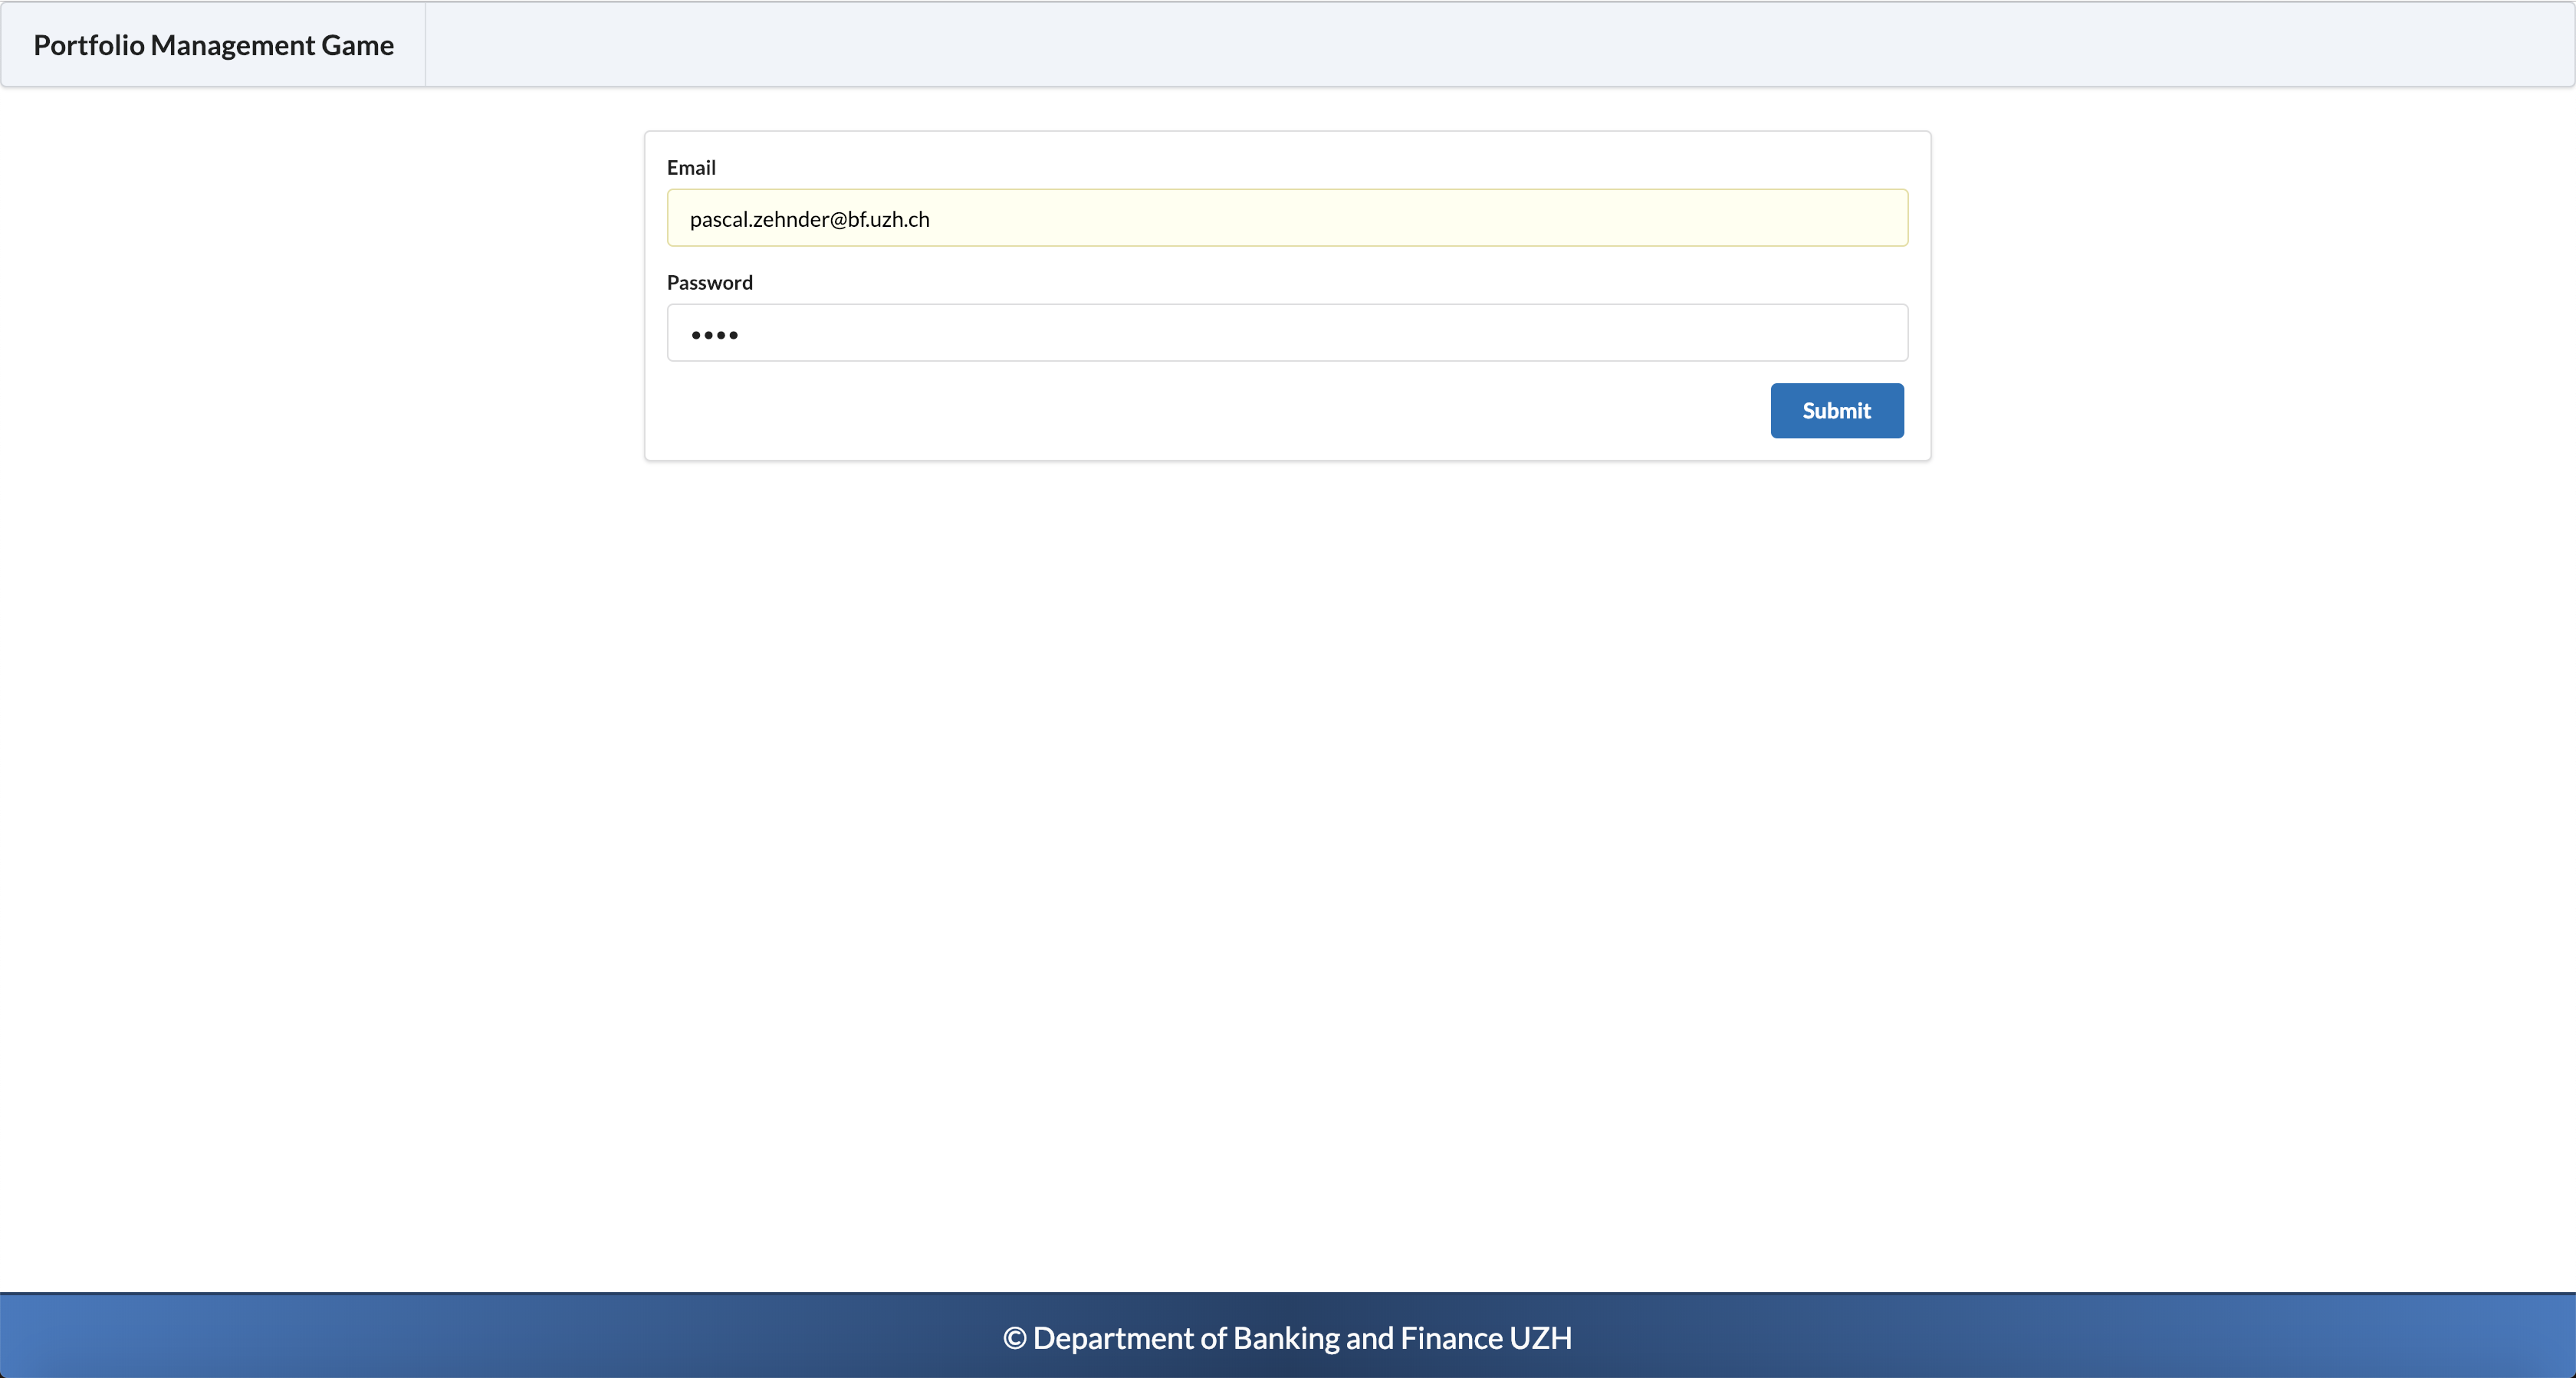
\includegraphics[scale=0.2]{img/application-overview/administrator/login.png}
\end{center}

\subsubsection{Game management}
\paragraph{Game overview}
As landing page of the administrator the game overview exists. It serves as the control center of the game adminstration.
\begin{center}
  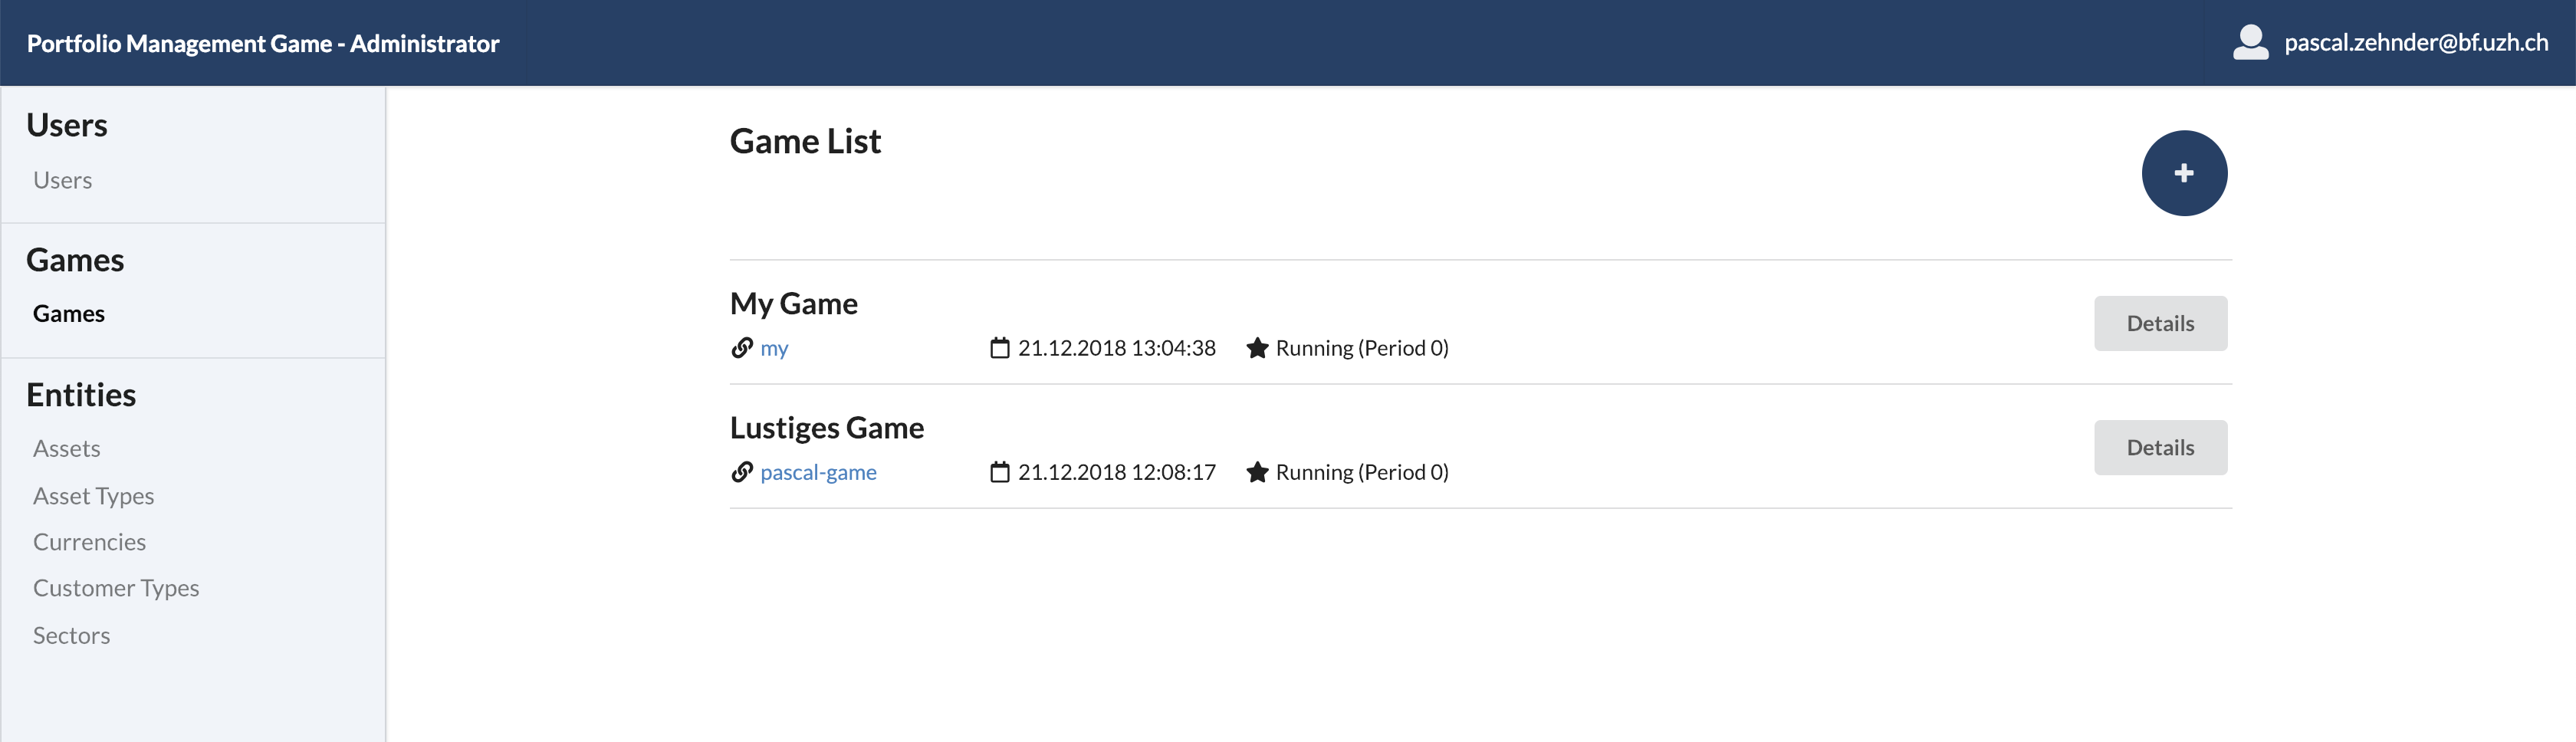
\includegraphics[scale=0.2]{img/application-overview/administrator/game_overview.png}
\end{center}

\paragraph{Game creation}
For creating a game the administrator needs to define some parameters for playing a game which are structured into three tabs. By pressing on the ''next''-button the administrator will be leaded through the form. Some tooltips help users to understand the purpose of the provided input. After submitting the creation of the game, the user will be redirected to the game overview.
\begin{center}
  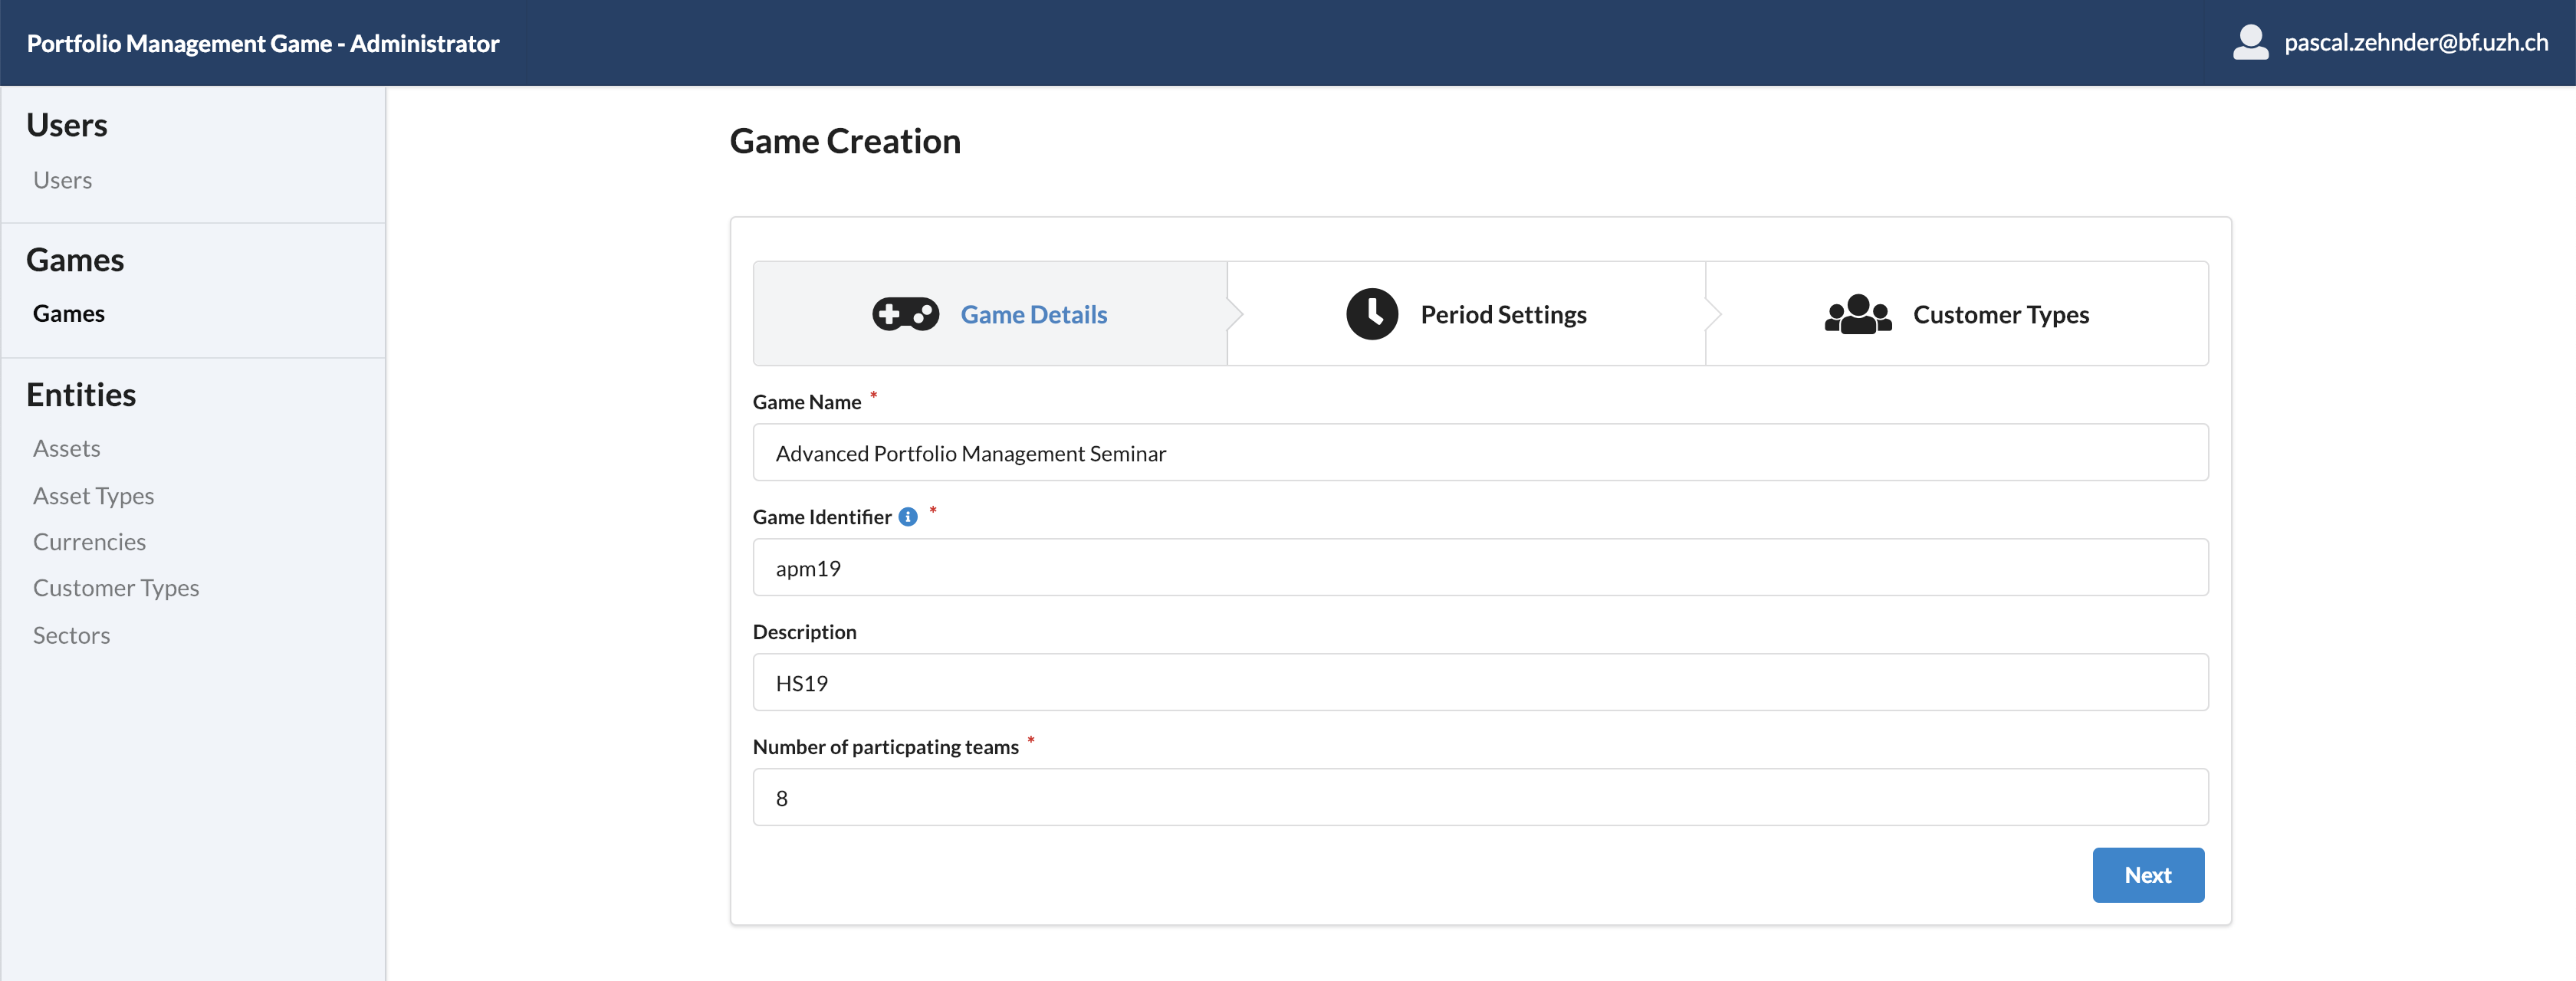
\includegraphics[scale=0.2]{img/application-overview/administrator/game_creation.png}
\end{center}

\paragraph{Game detail}
The game detail for each game may be accessed over the game overview list. In this page a user can intialize period, start periods, having an overview about the teams submission and many other features, which will be described in this part:

\subparagraph{Game initialization}
As the game creation may be done in advance we have splitten the game creation from the game initialization, such that last adjustments of the game may be done just before the start of the game.
\begin{center}
  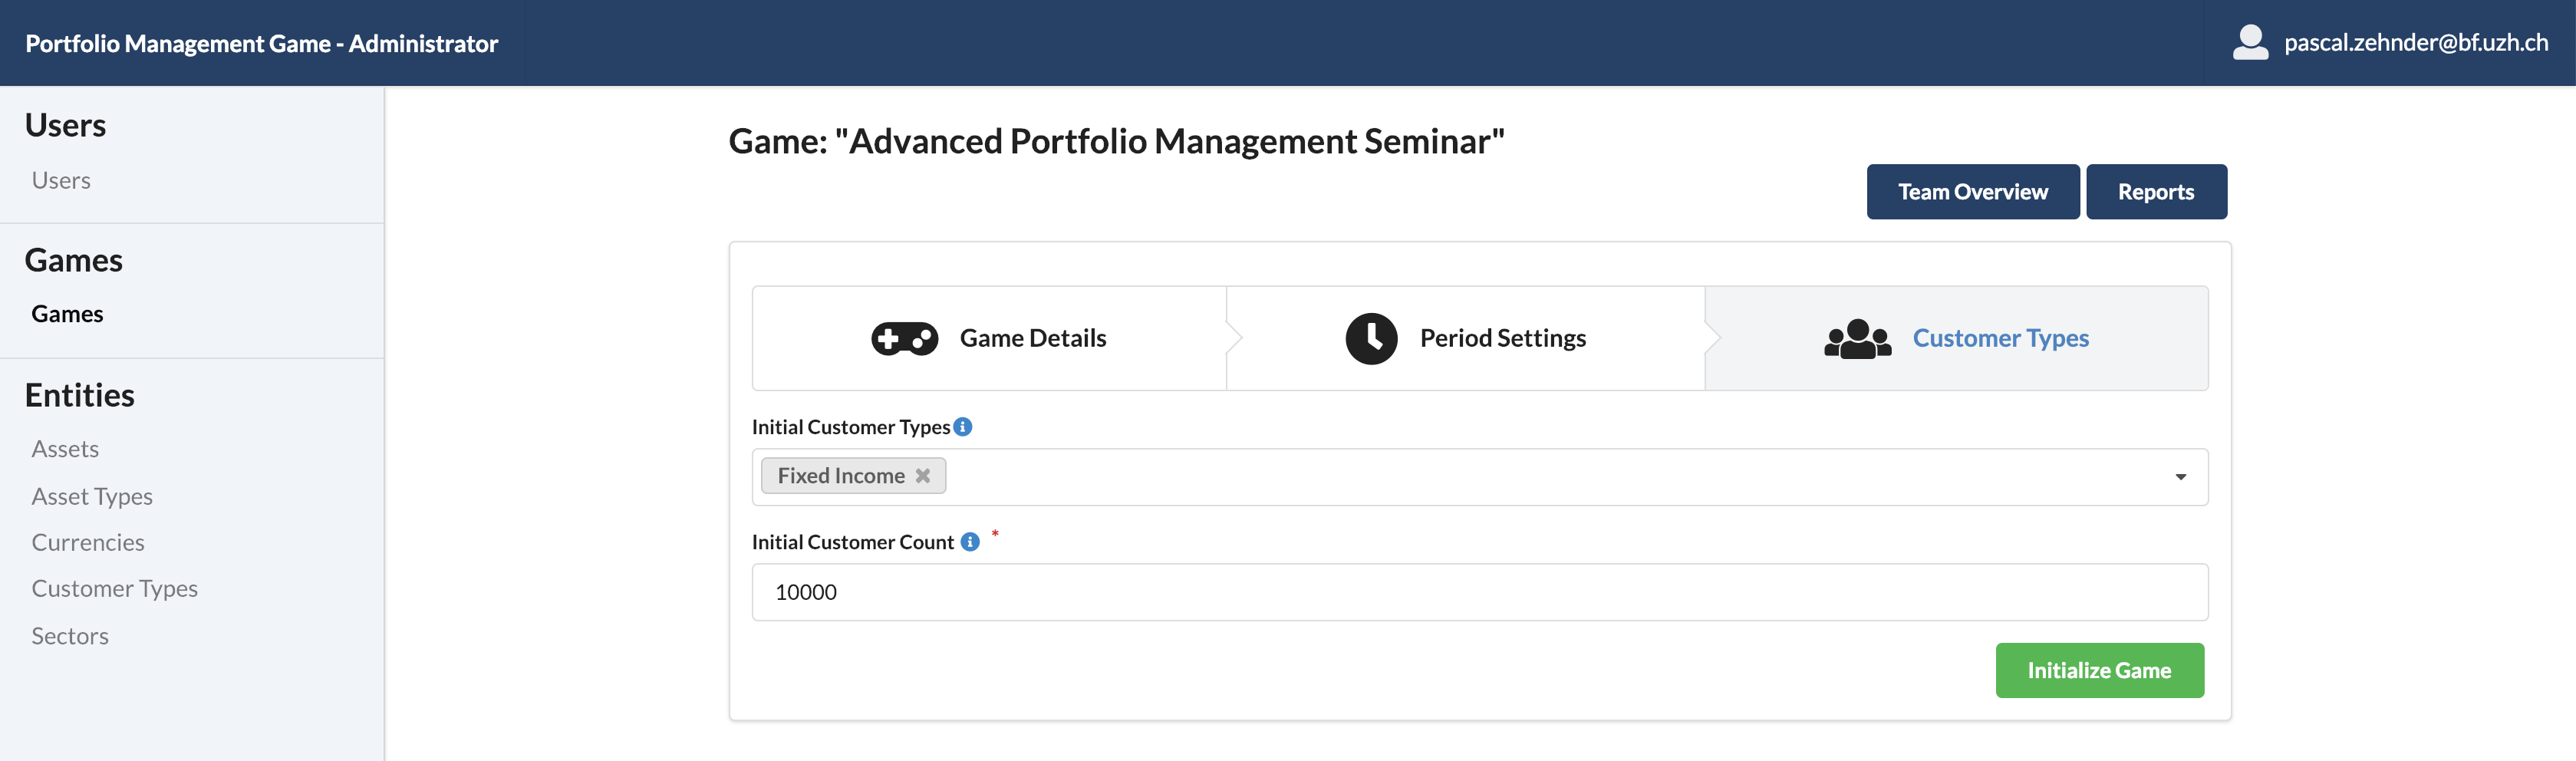
\includegraphics[scale=0.2]{img/application-overview/administrator/game_initialization.png}
\end{center}

\subparagraph{Game start}
By starting the game the students or teams are finally able to start with their period 0 decisions. Administrators are able to give them some help over messages which will be visible for the teams in their report section.
\begin{center}
  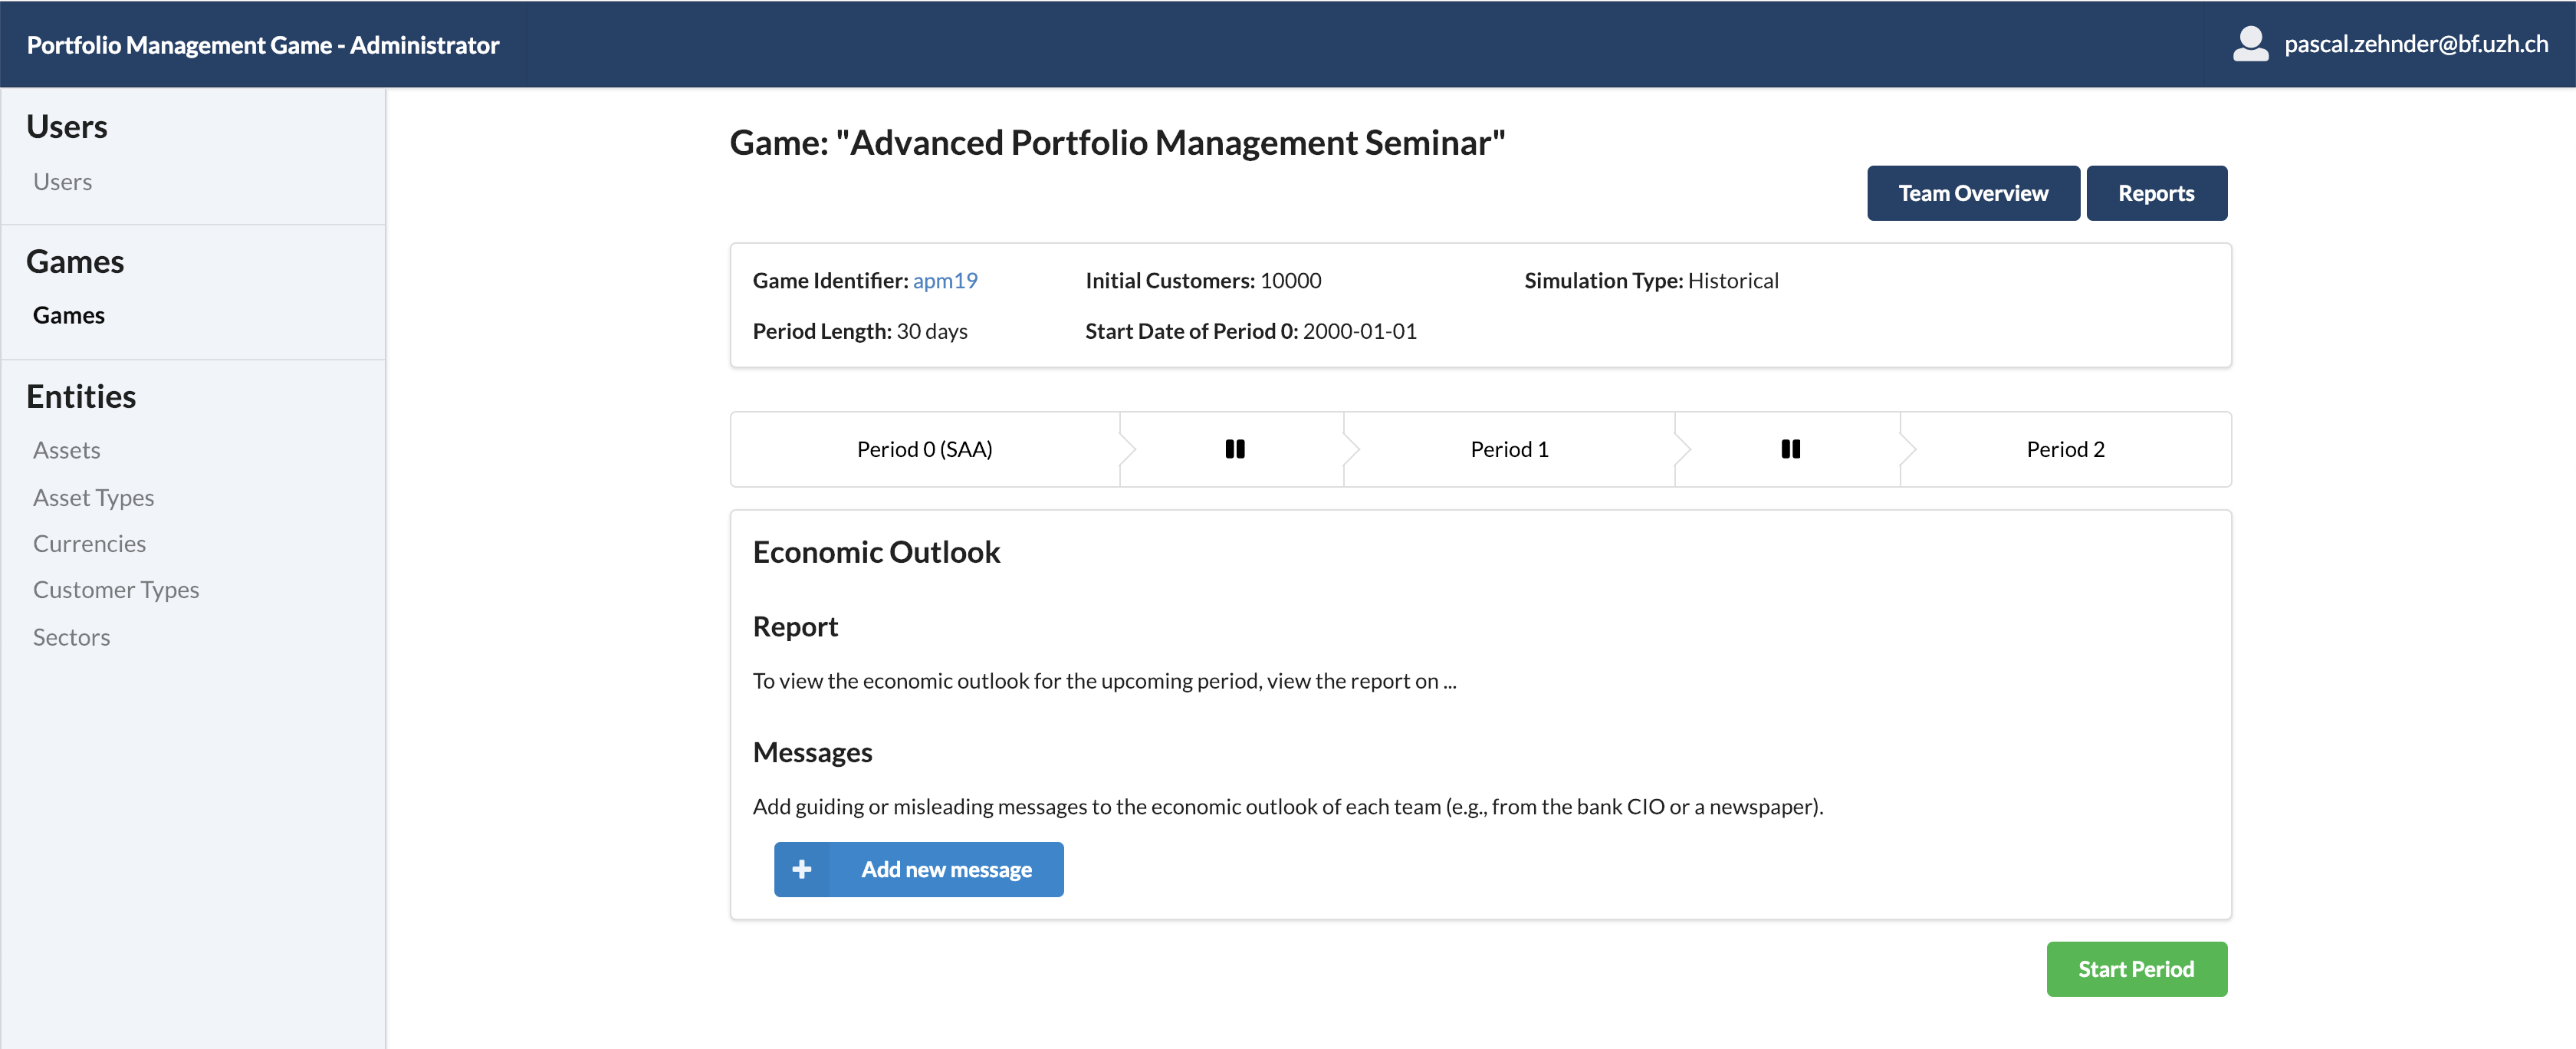
\includegraphics[scale=0.2]{img/application-overview/administrator/game_start.png}
\end{center}

\subparagraph{Team overview}
For providing access for all teams an administrator has an overview about the team logins, which are generated automatically when initializing the game.
\begin{center}
  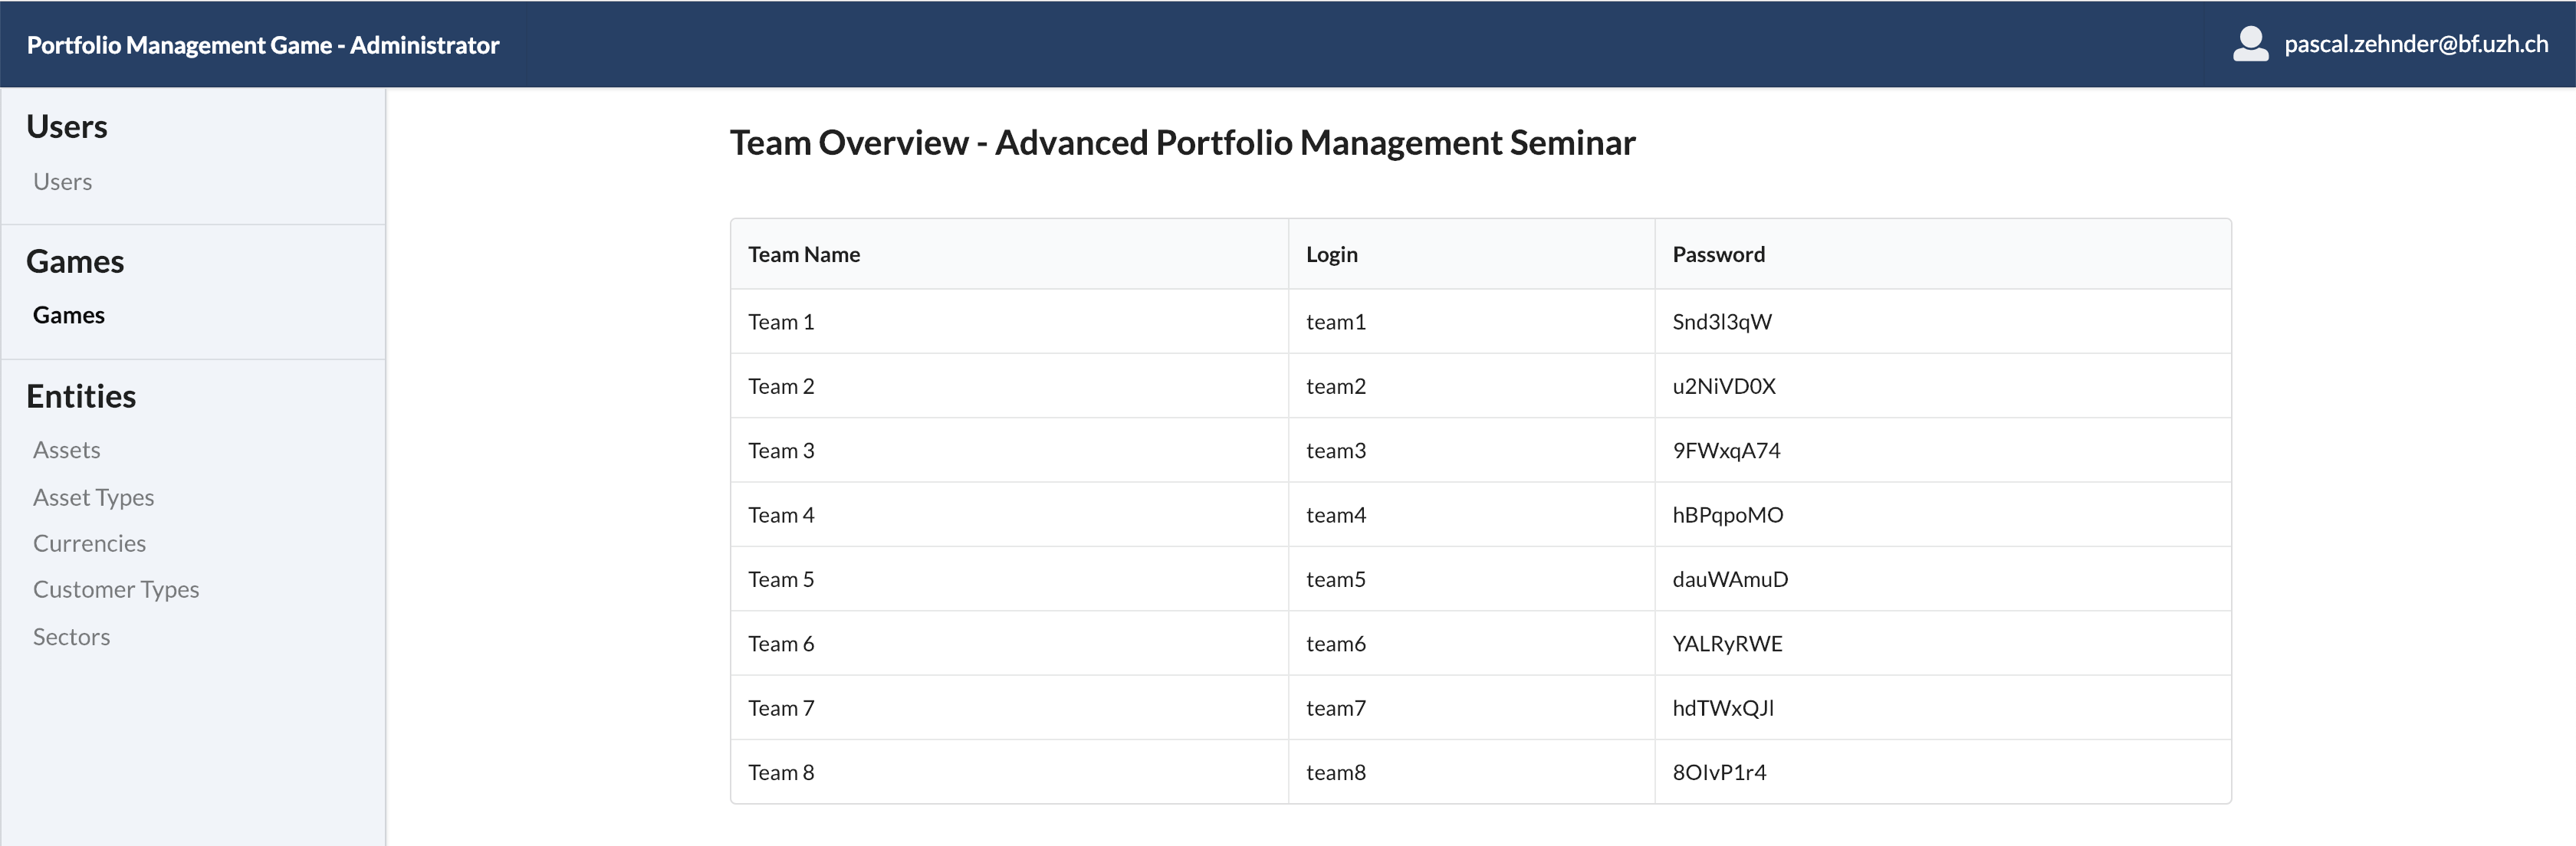
\includegraphics[scale=0.2]{img/application-overview/administrator/team_login_overview.png}
\end{center}

\subparagraph{Running game}
Overview about the submission state of all teams. The administrator is able to get an insight about the decisions of all submitted teams. The period can only be finished if all teams submitted and therefore the state of the teams has been green.
\begin{center}
  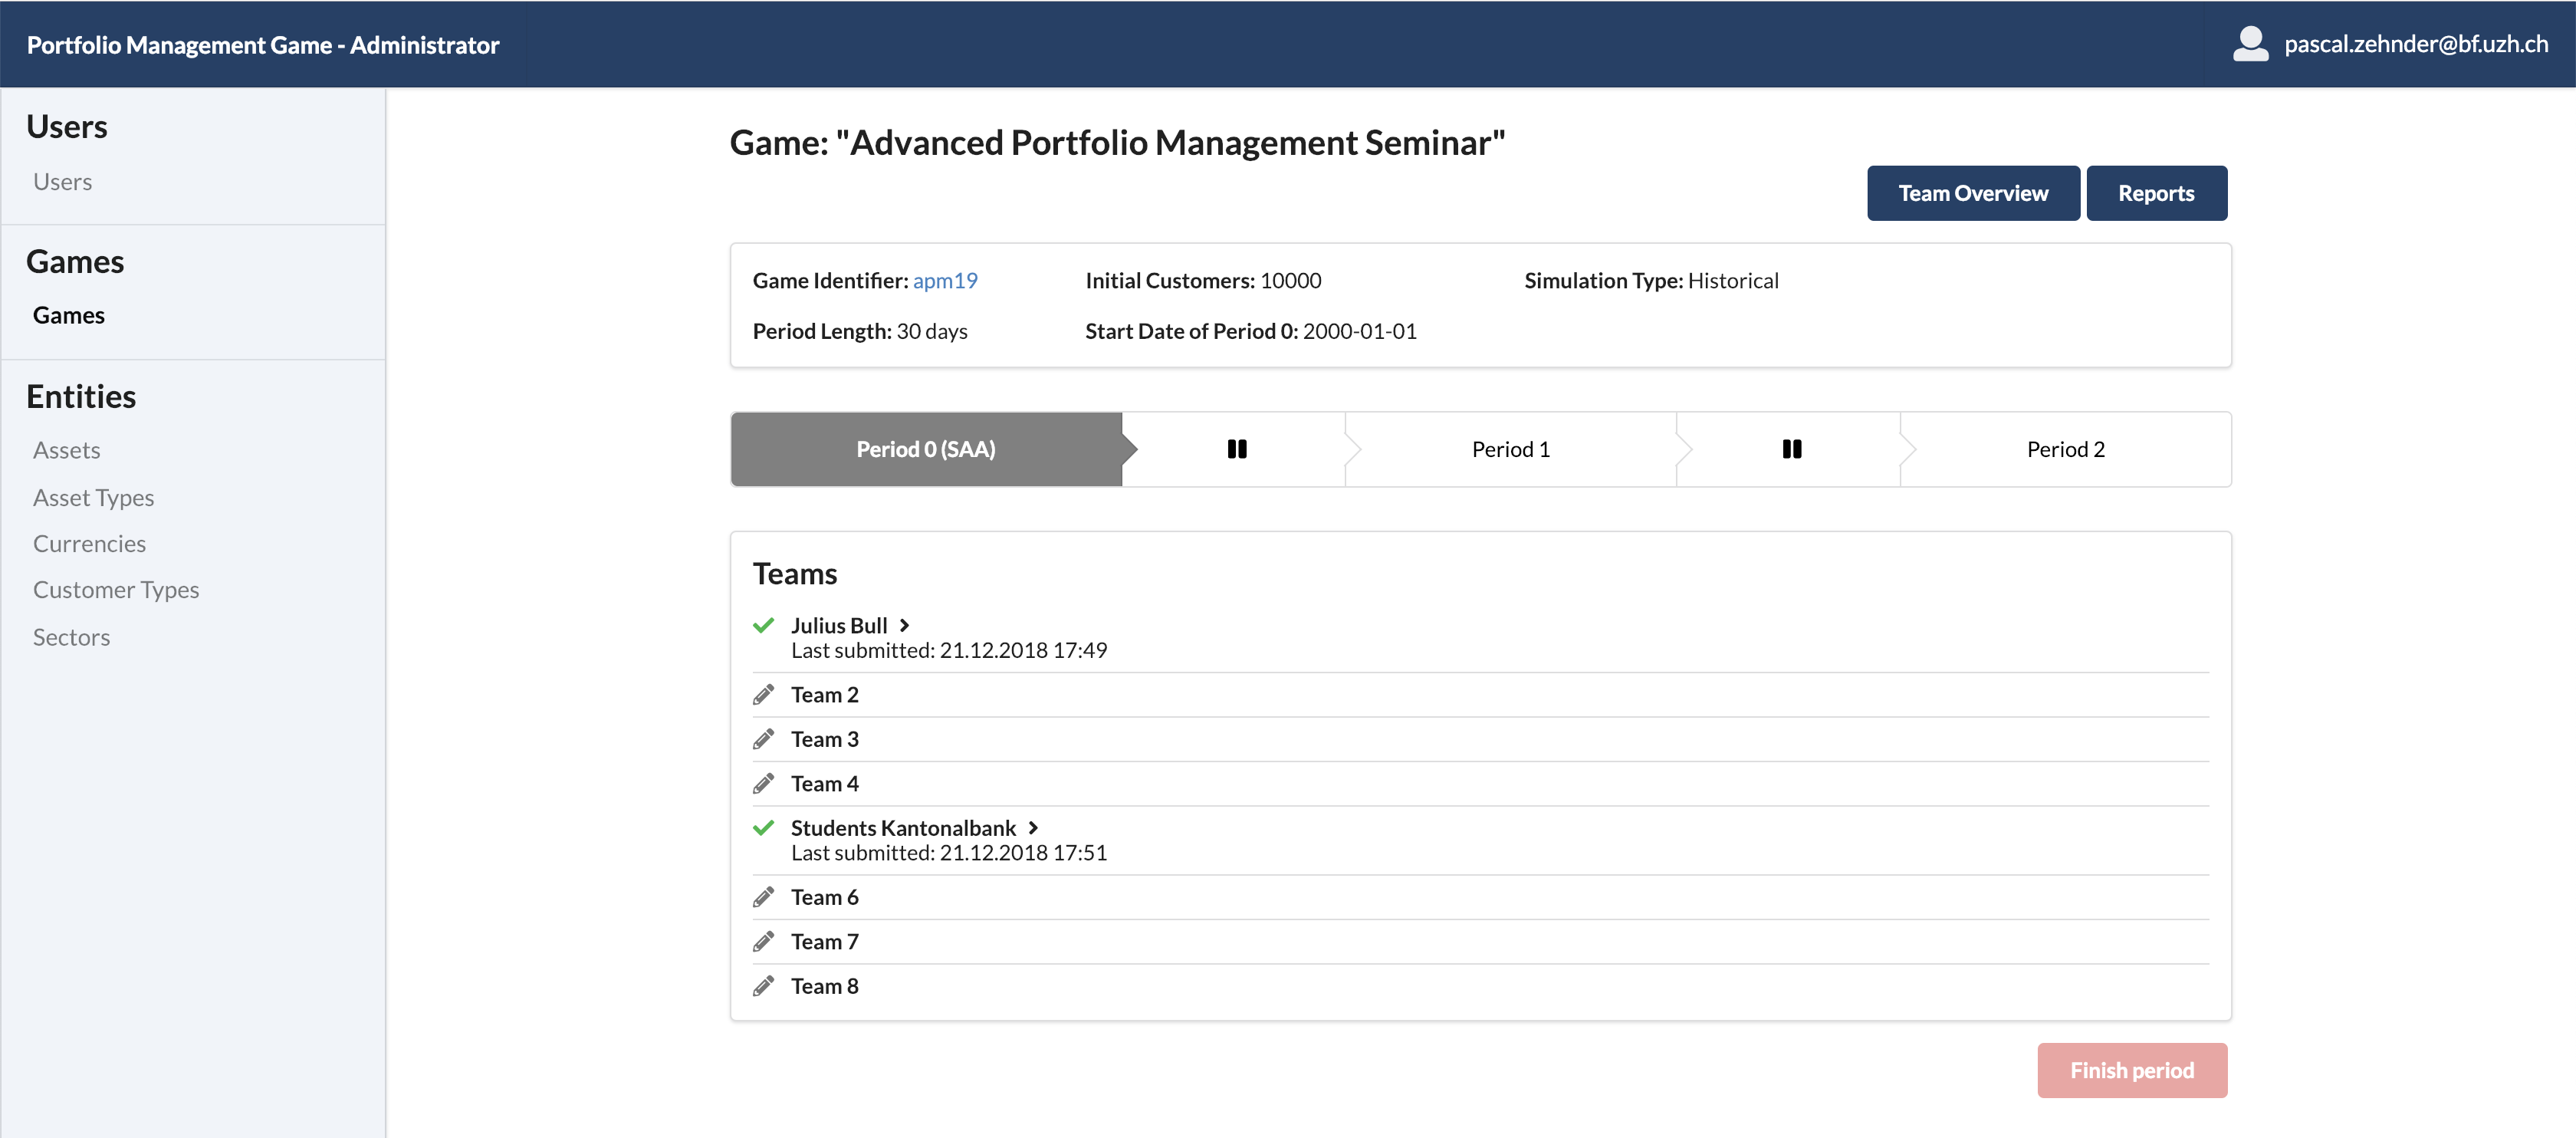
\includegraphics[scale=0.2]{img/application-overview/administrator/running_game.png}
\end{center}

\subparagraph{Initializing period}
After completion of period zero the administrator has to initalize a period in which the team decisions will be compared to the other teams decisions and evaluated. Additionally new customer types for the next period and other settings could be defined in this phase of the game.
% TODO replace with screen including customer type settings
\begin{center}
  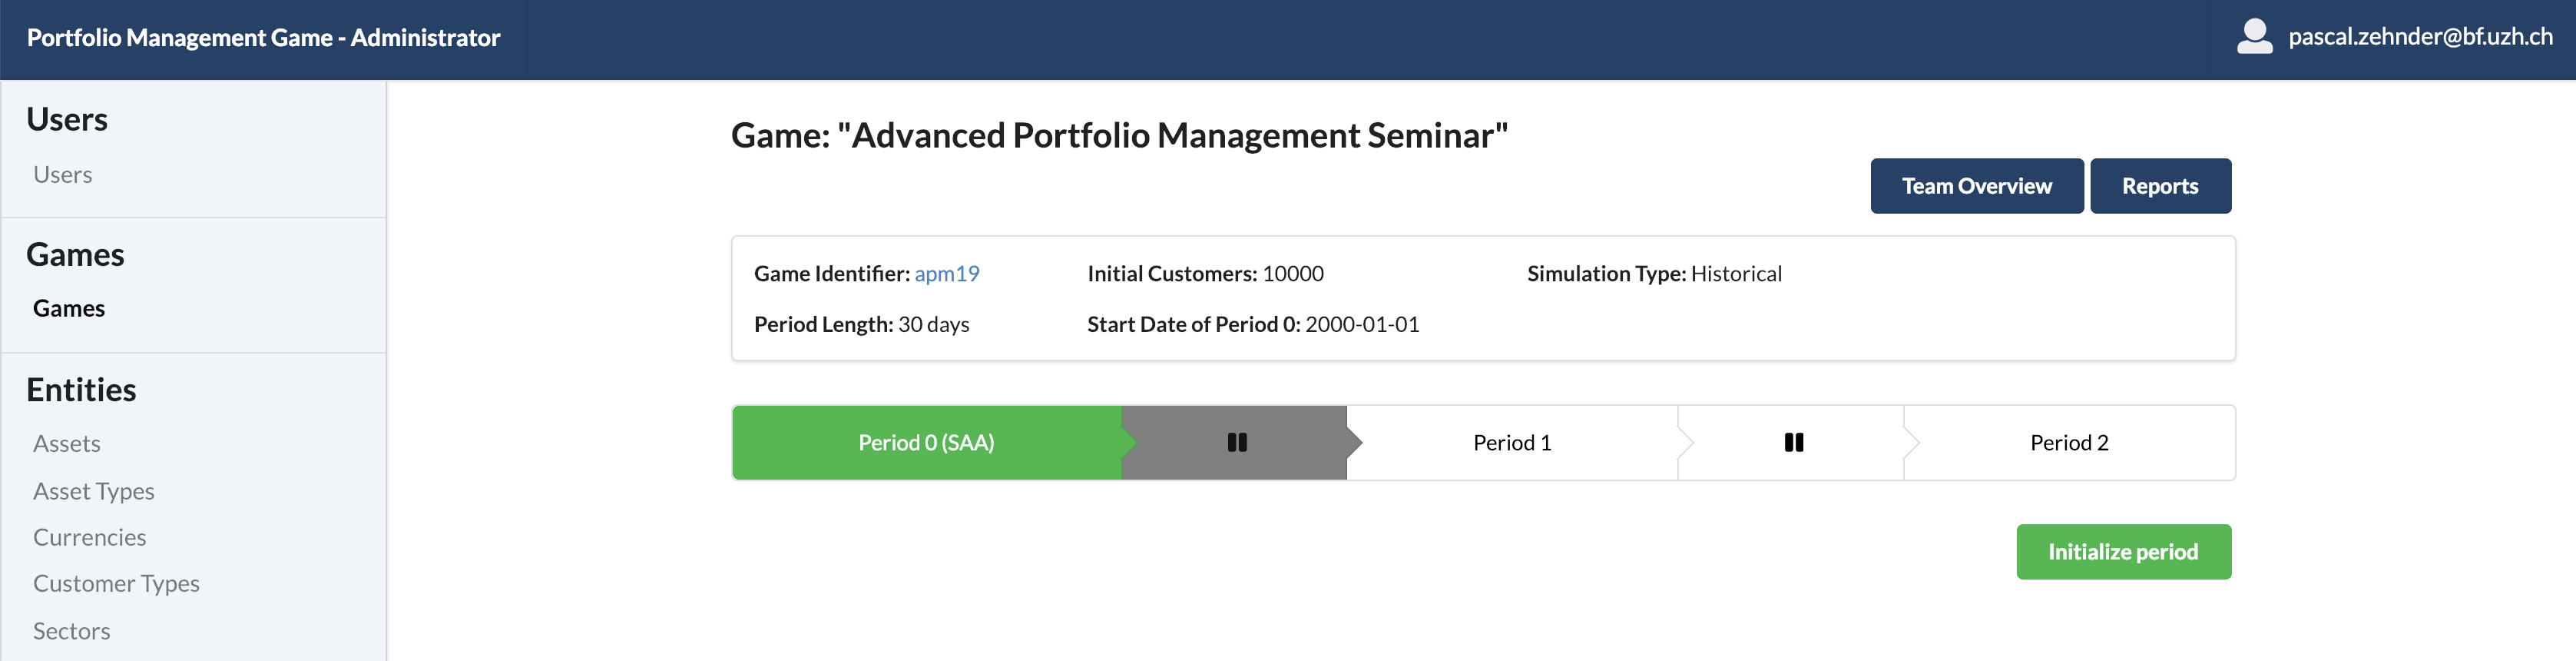
\includegraphics[scale=0.2]{img/application-overview/administrator/period_initialization.png}
\end{center}

\subparagraph{Period start}
By completing the simulation, respectively evaluation of the previous period, a next period may be started. If the game is still paused the teams cannot access the decisions site. The administrator can define some optional messages which will be displayed in the teams report page. Some adjustments to the simulation results will be edited in this phase of the game.
\begin{center}
  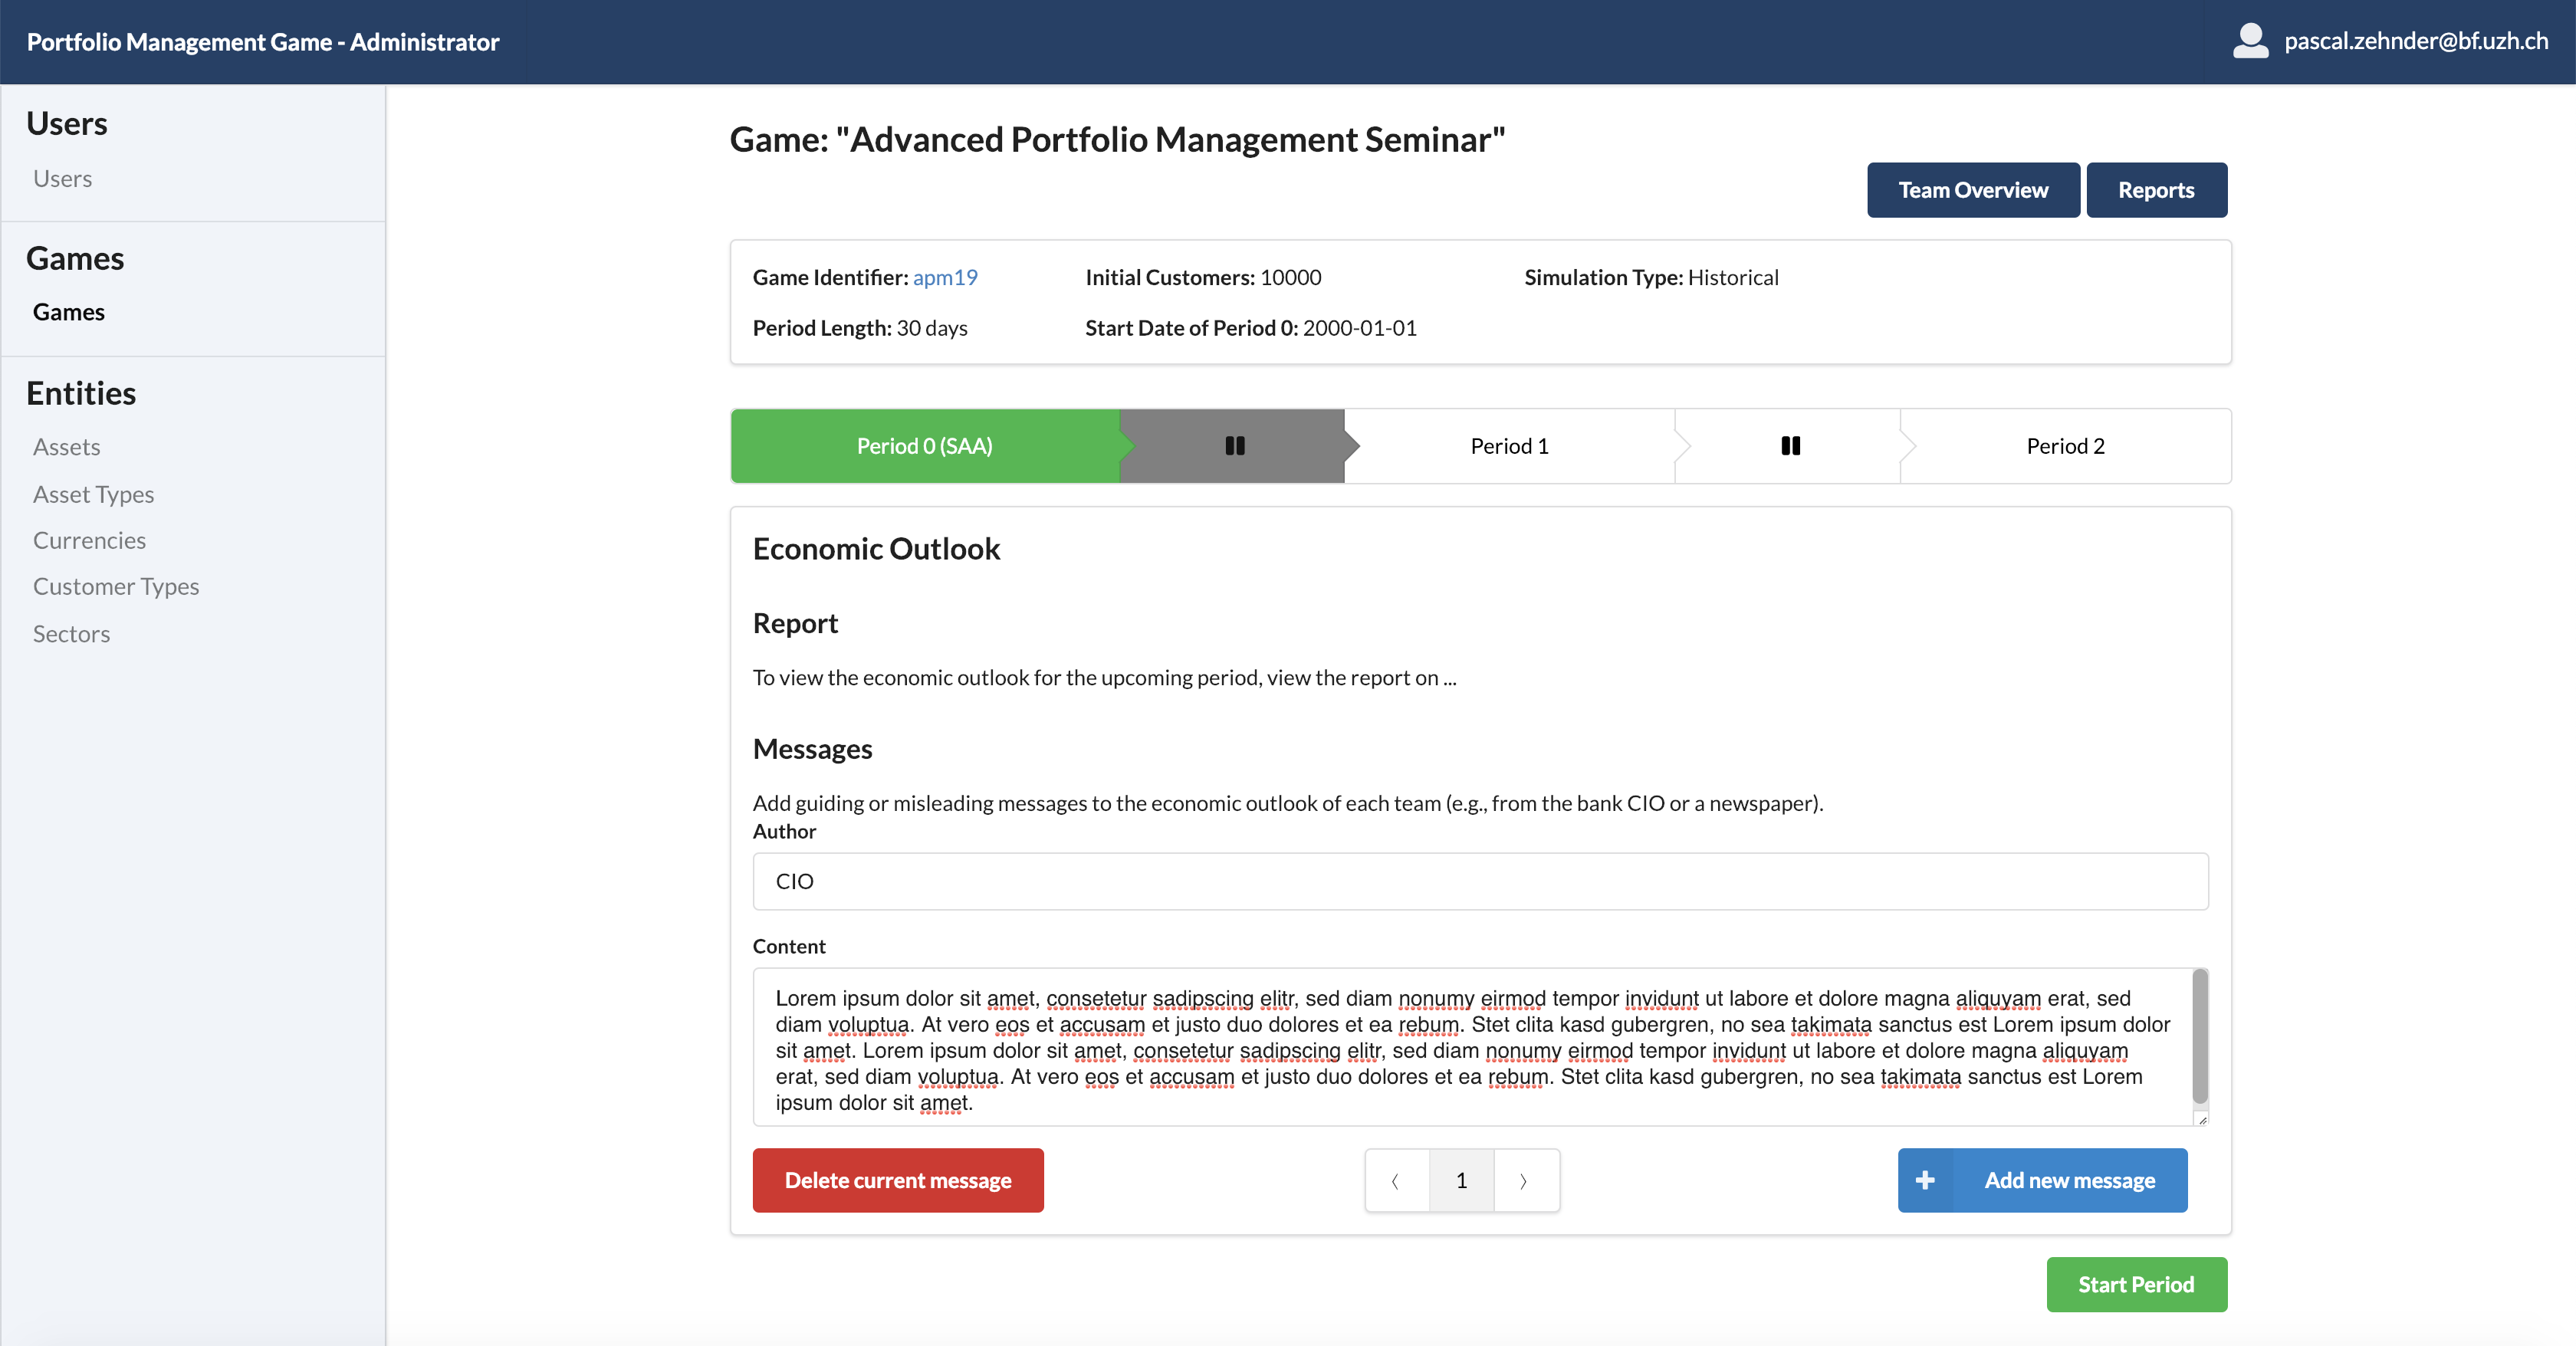
\includegraphics[scale=0.2]{img/application-overview/administrator/period_start.png}
\end{center}

\subsubsection{Entities adminitration}

\paragraph{Assets}
\begin{center}
  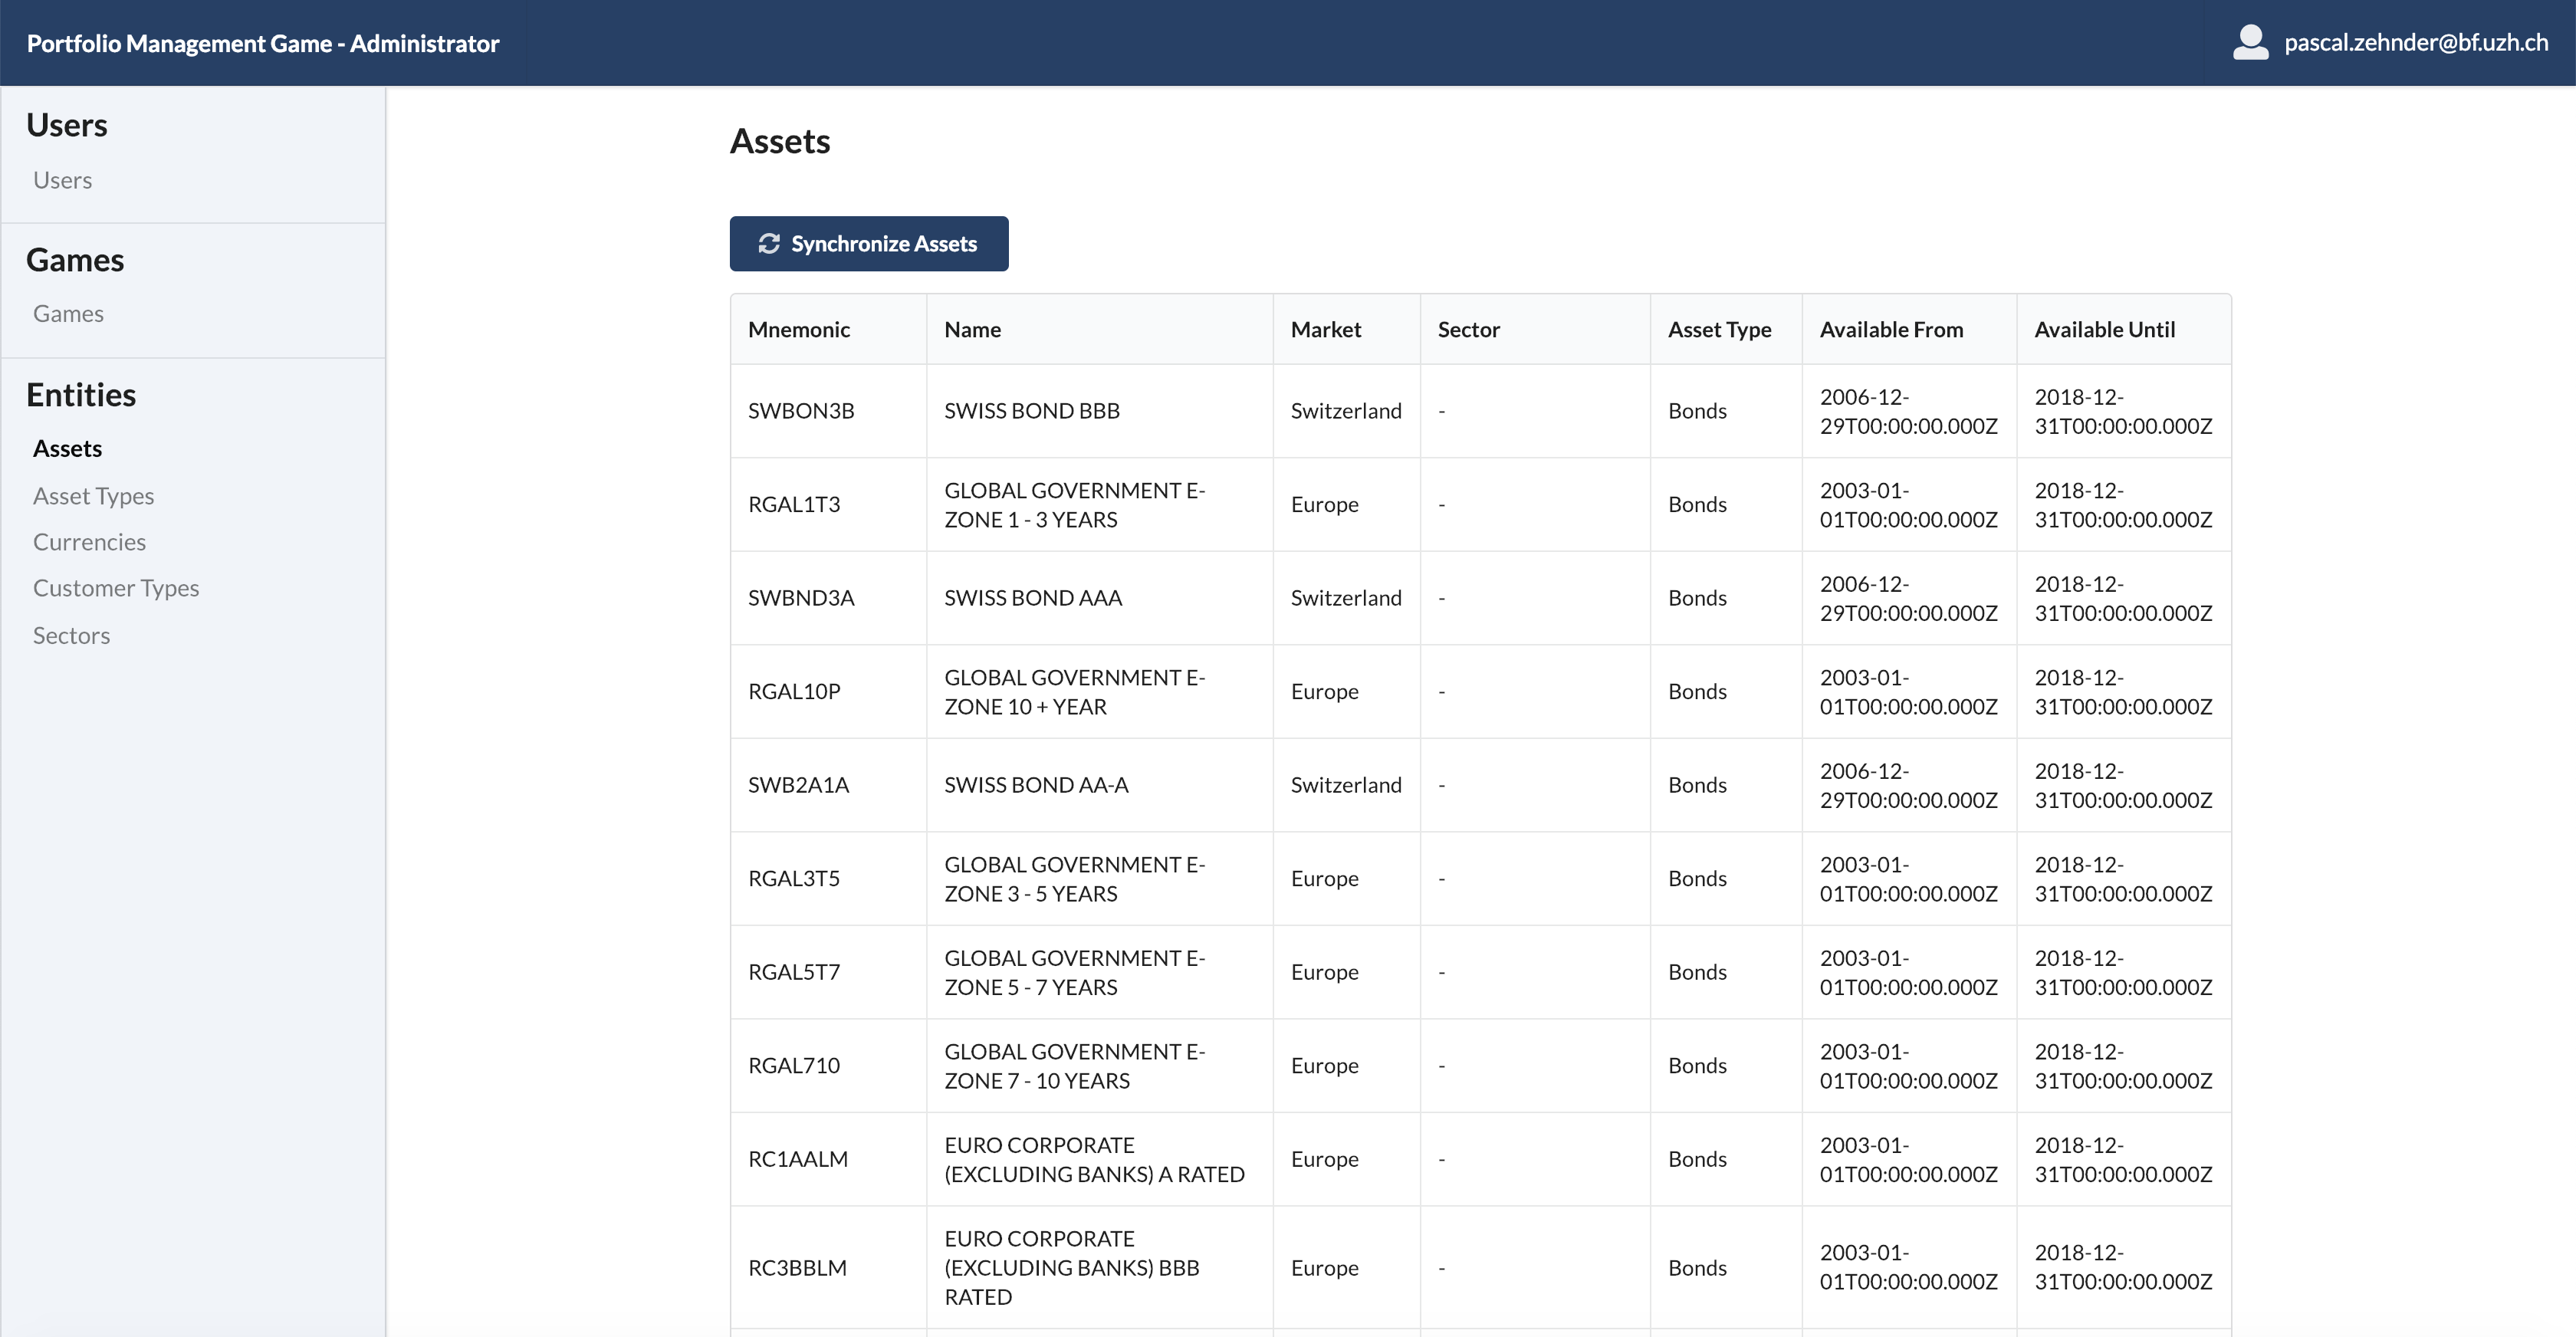
\includegraphics[scale=0.2]{img/application-overview/administrator/entities_assets.png}
\end{center}

\paragraph{Asset Types}
A table showing all asset types which may be edited is the landing page of this entity. By editing a specified asset type the administrator can change some characteristics of its type, such as info text.
\begin{center}
  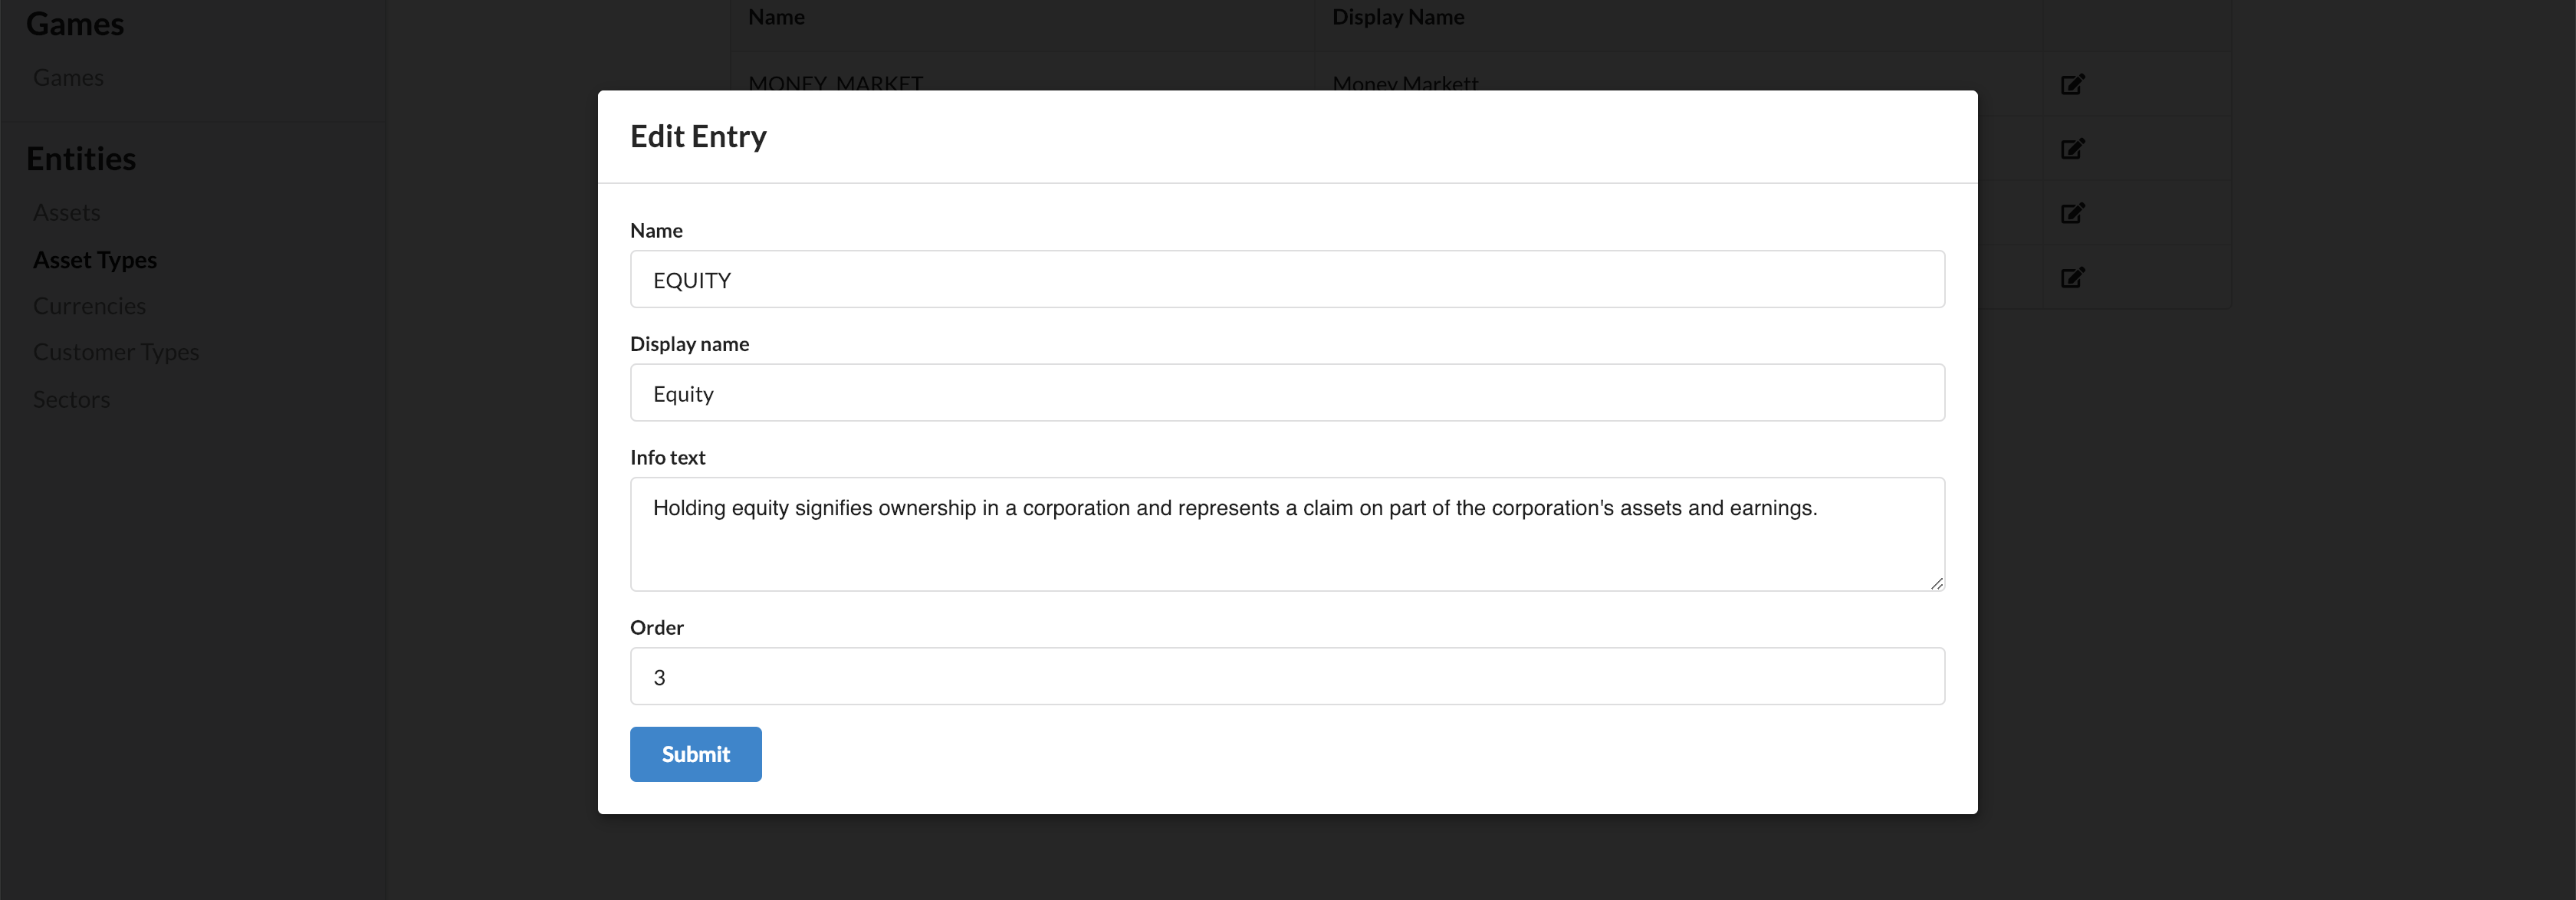
\includegraphics[scale=0.2]{img/application-overview/administrator/entities_asset_types.png}
\end{center}

\paragraph{Currencies}
The currencies may be edited in a same manner as the asset types.

\paragraph{Customer Types}
An overview about all in the game available customer types is provided for the administrator. For each customer type the ideal strategic asset allocation and the ranges for currencies and asset types (both dimensions) can be modified. Additionaly the info bullets and the displaying name may be modified too.
\begin{center}
  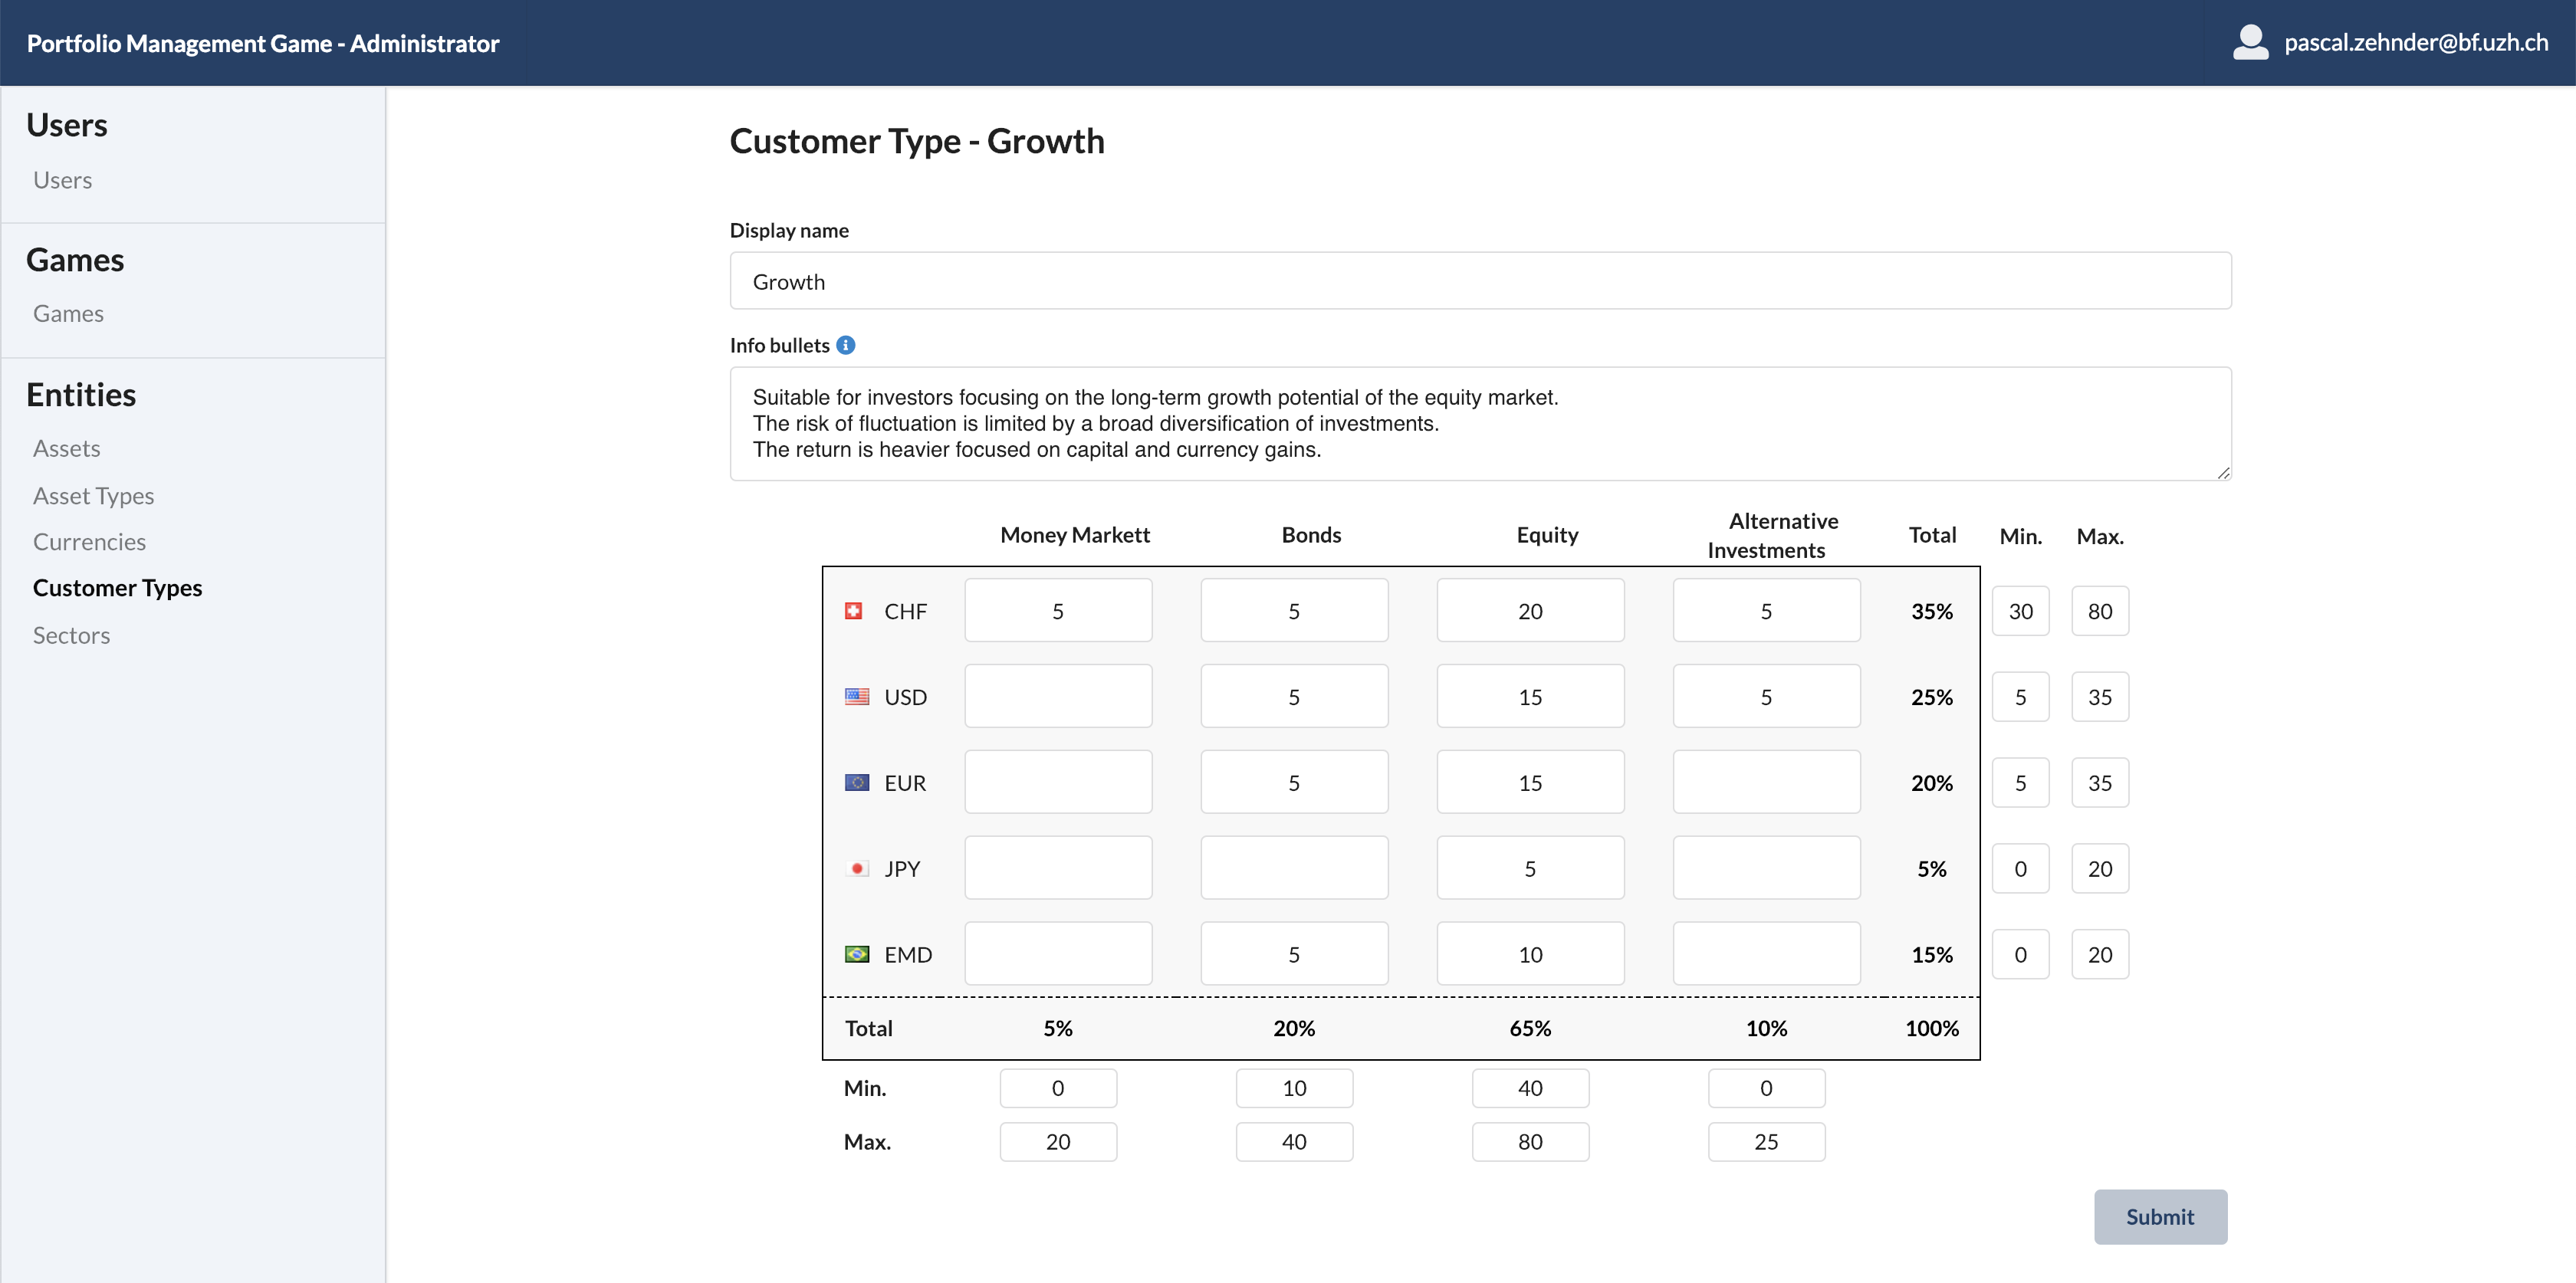
\includegraphics[scale=0.2]{img/application-overview/administrator/entities_customer_types.png}
\end{center}

\paragraph{Sectors}
Short overview about all sectors which are used in the asset overview.







\subsection{Team View}

\subsubsection{Login}
\begin{center}
  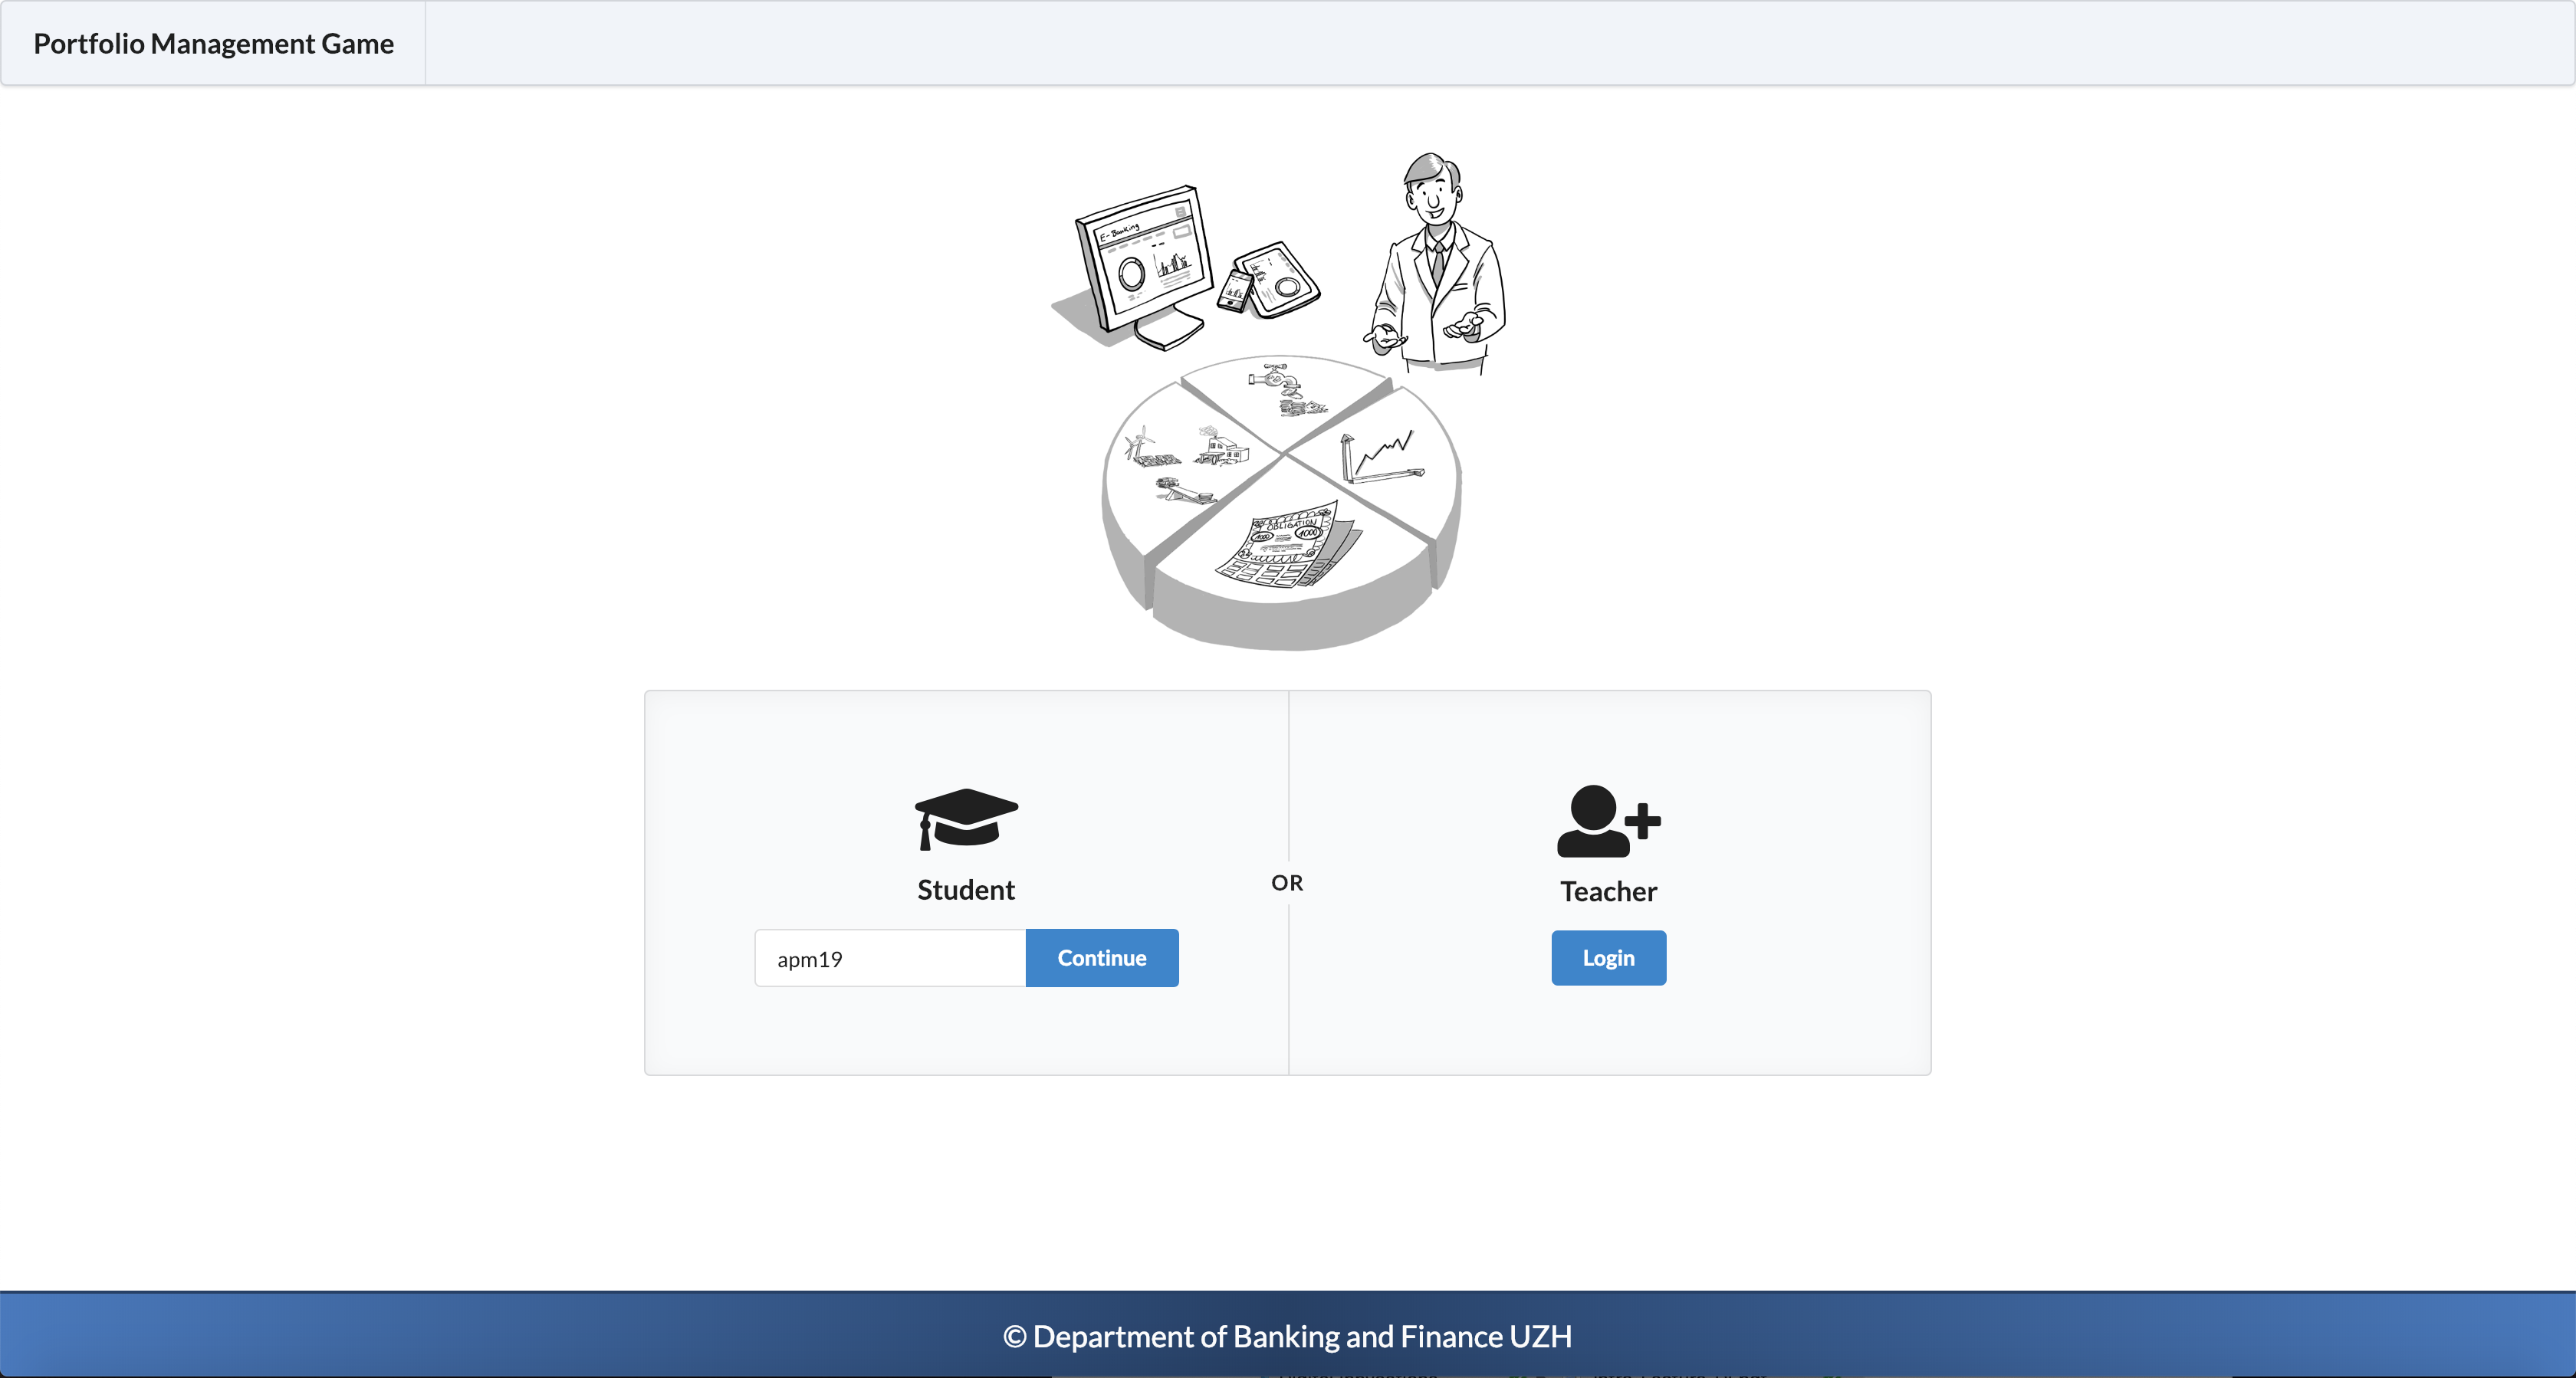
\includegraphics[scale=0.2]{img/application-overview/teams/startpage.png}
\end{center}
\begin{center}
  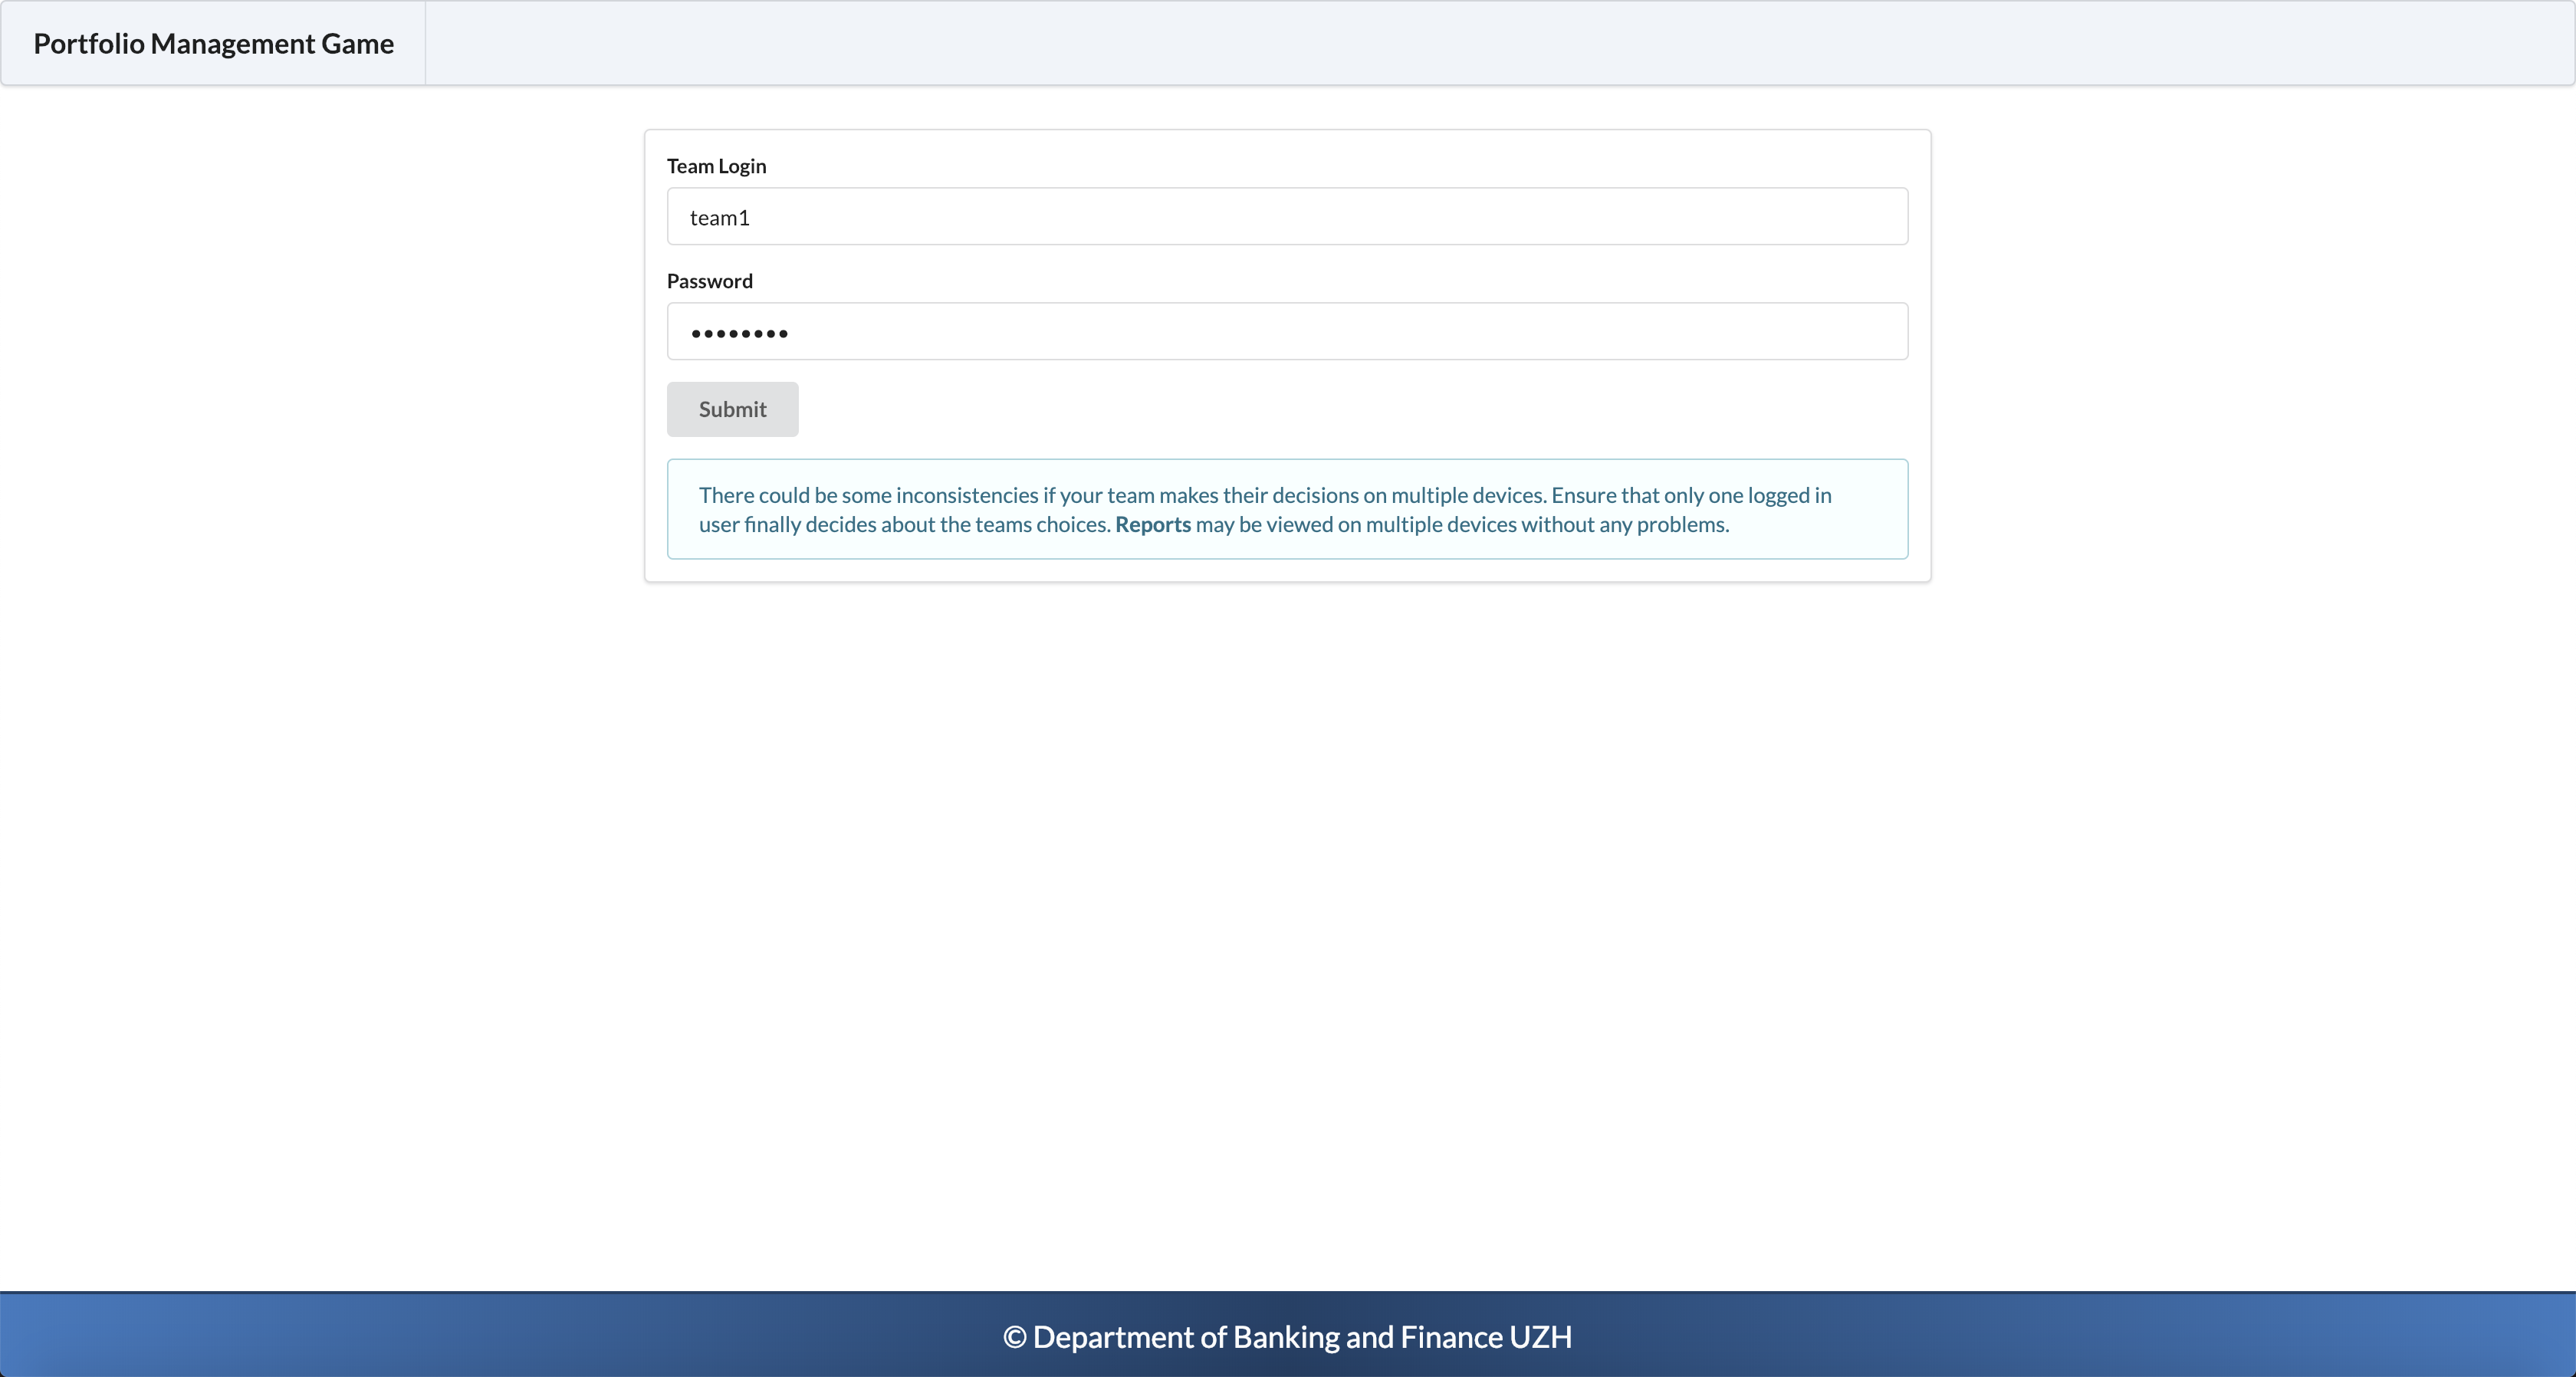
\includegraphics[scale=0.2]{img/application-overview/teams/login.png}
\end{center}

\subsection{Period 0 decisions}
In period 0 which represents phase 1 of the game, the teams define their SAA for all customer types which are enabled by the administrator of the specific game. The teams need to fullfill the ranges for all dimensions to submit their decisions. Supportive graphs in form of pie charts help the teams to decide about the share of the two dimensions. Additionaly the players can name their team on the top left corner of the screen.
\begin{center}
  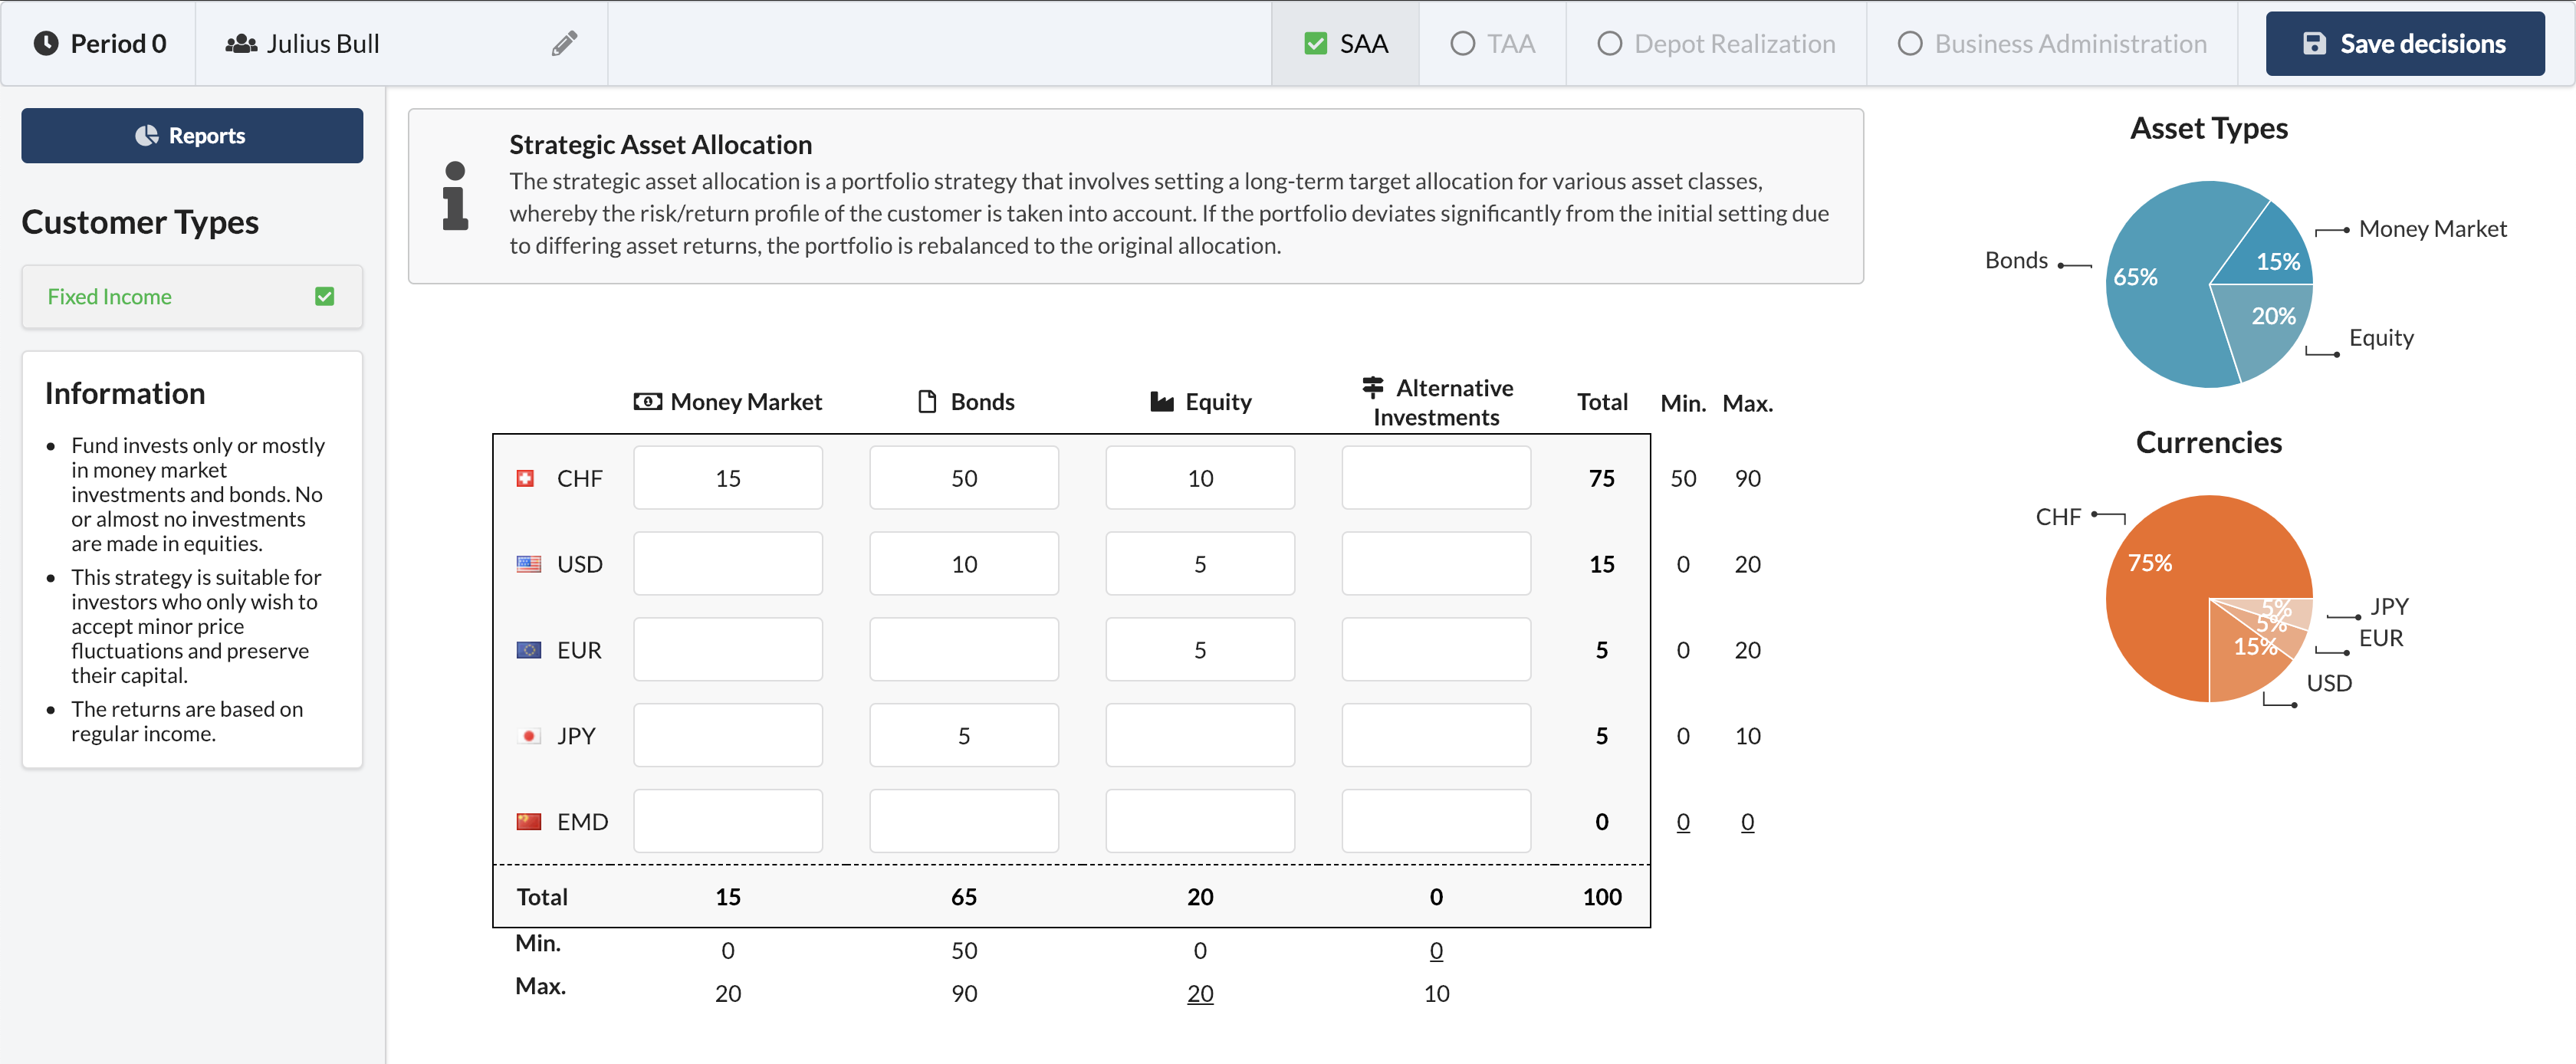
\includegraphics[scale=0.2]{img/application-overview/teams/period_zero_decisions.png}
\end{center}

\subsection{Other periods decisions}
\subsubsection{TAA}
\begin{center}
  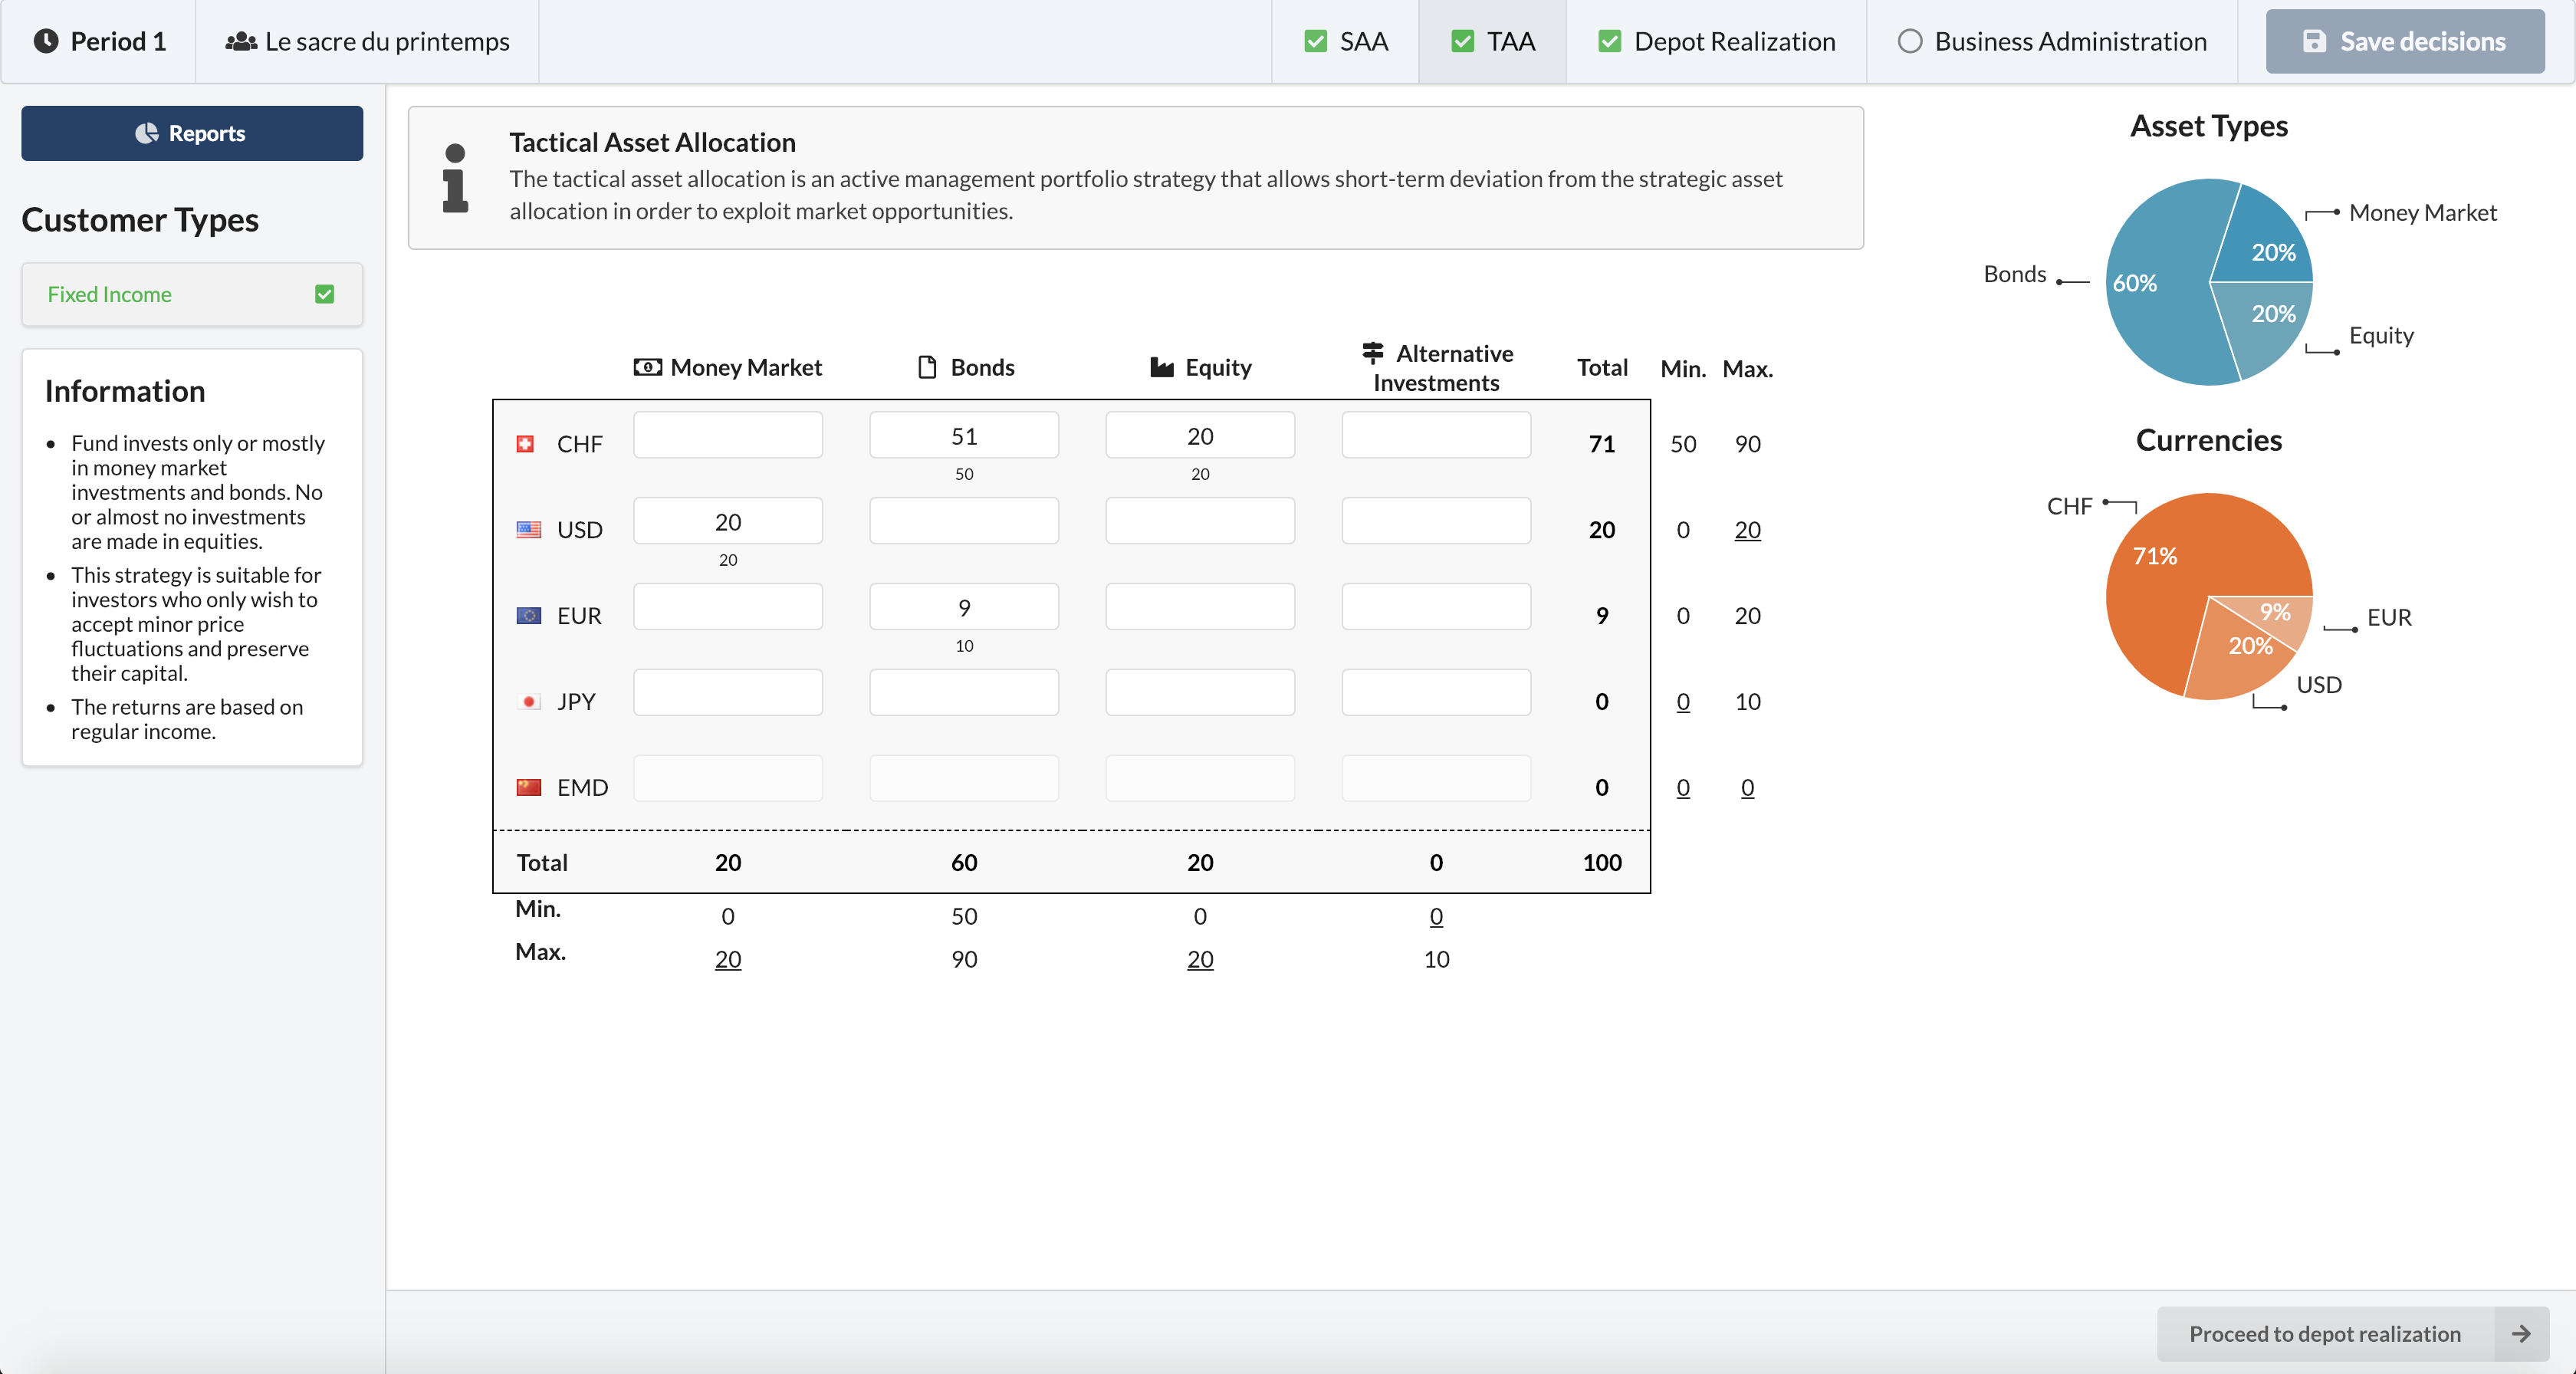
\includegraphics[scale=0.2]{img/application-overview/teams/taa.png}
\end{center}

\subsubsection{Depot Realization}
\begin{center}
  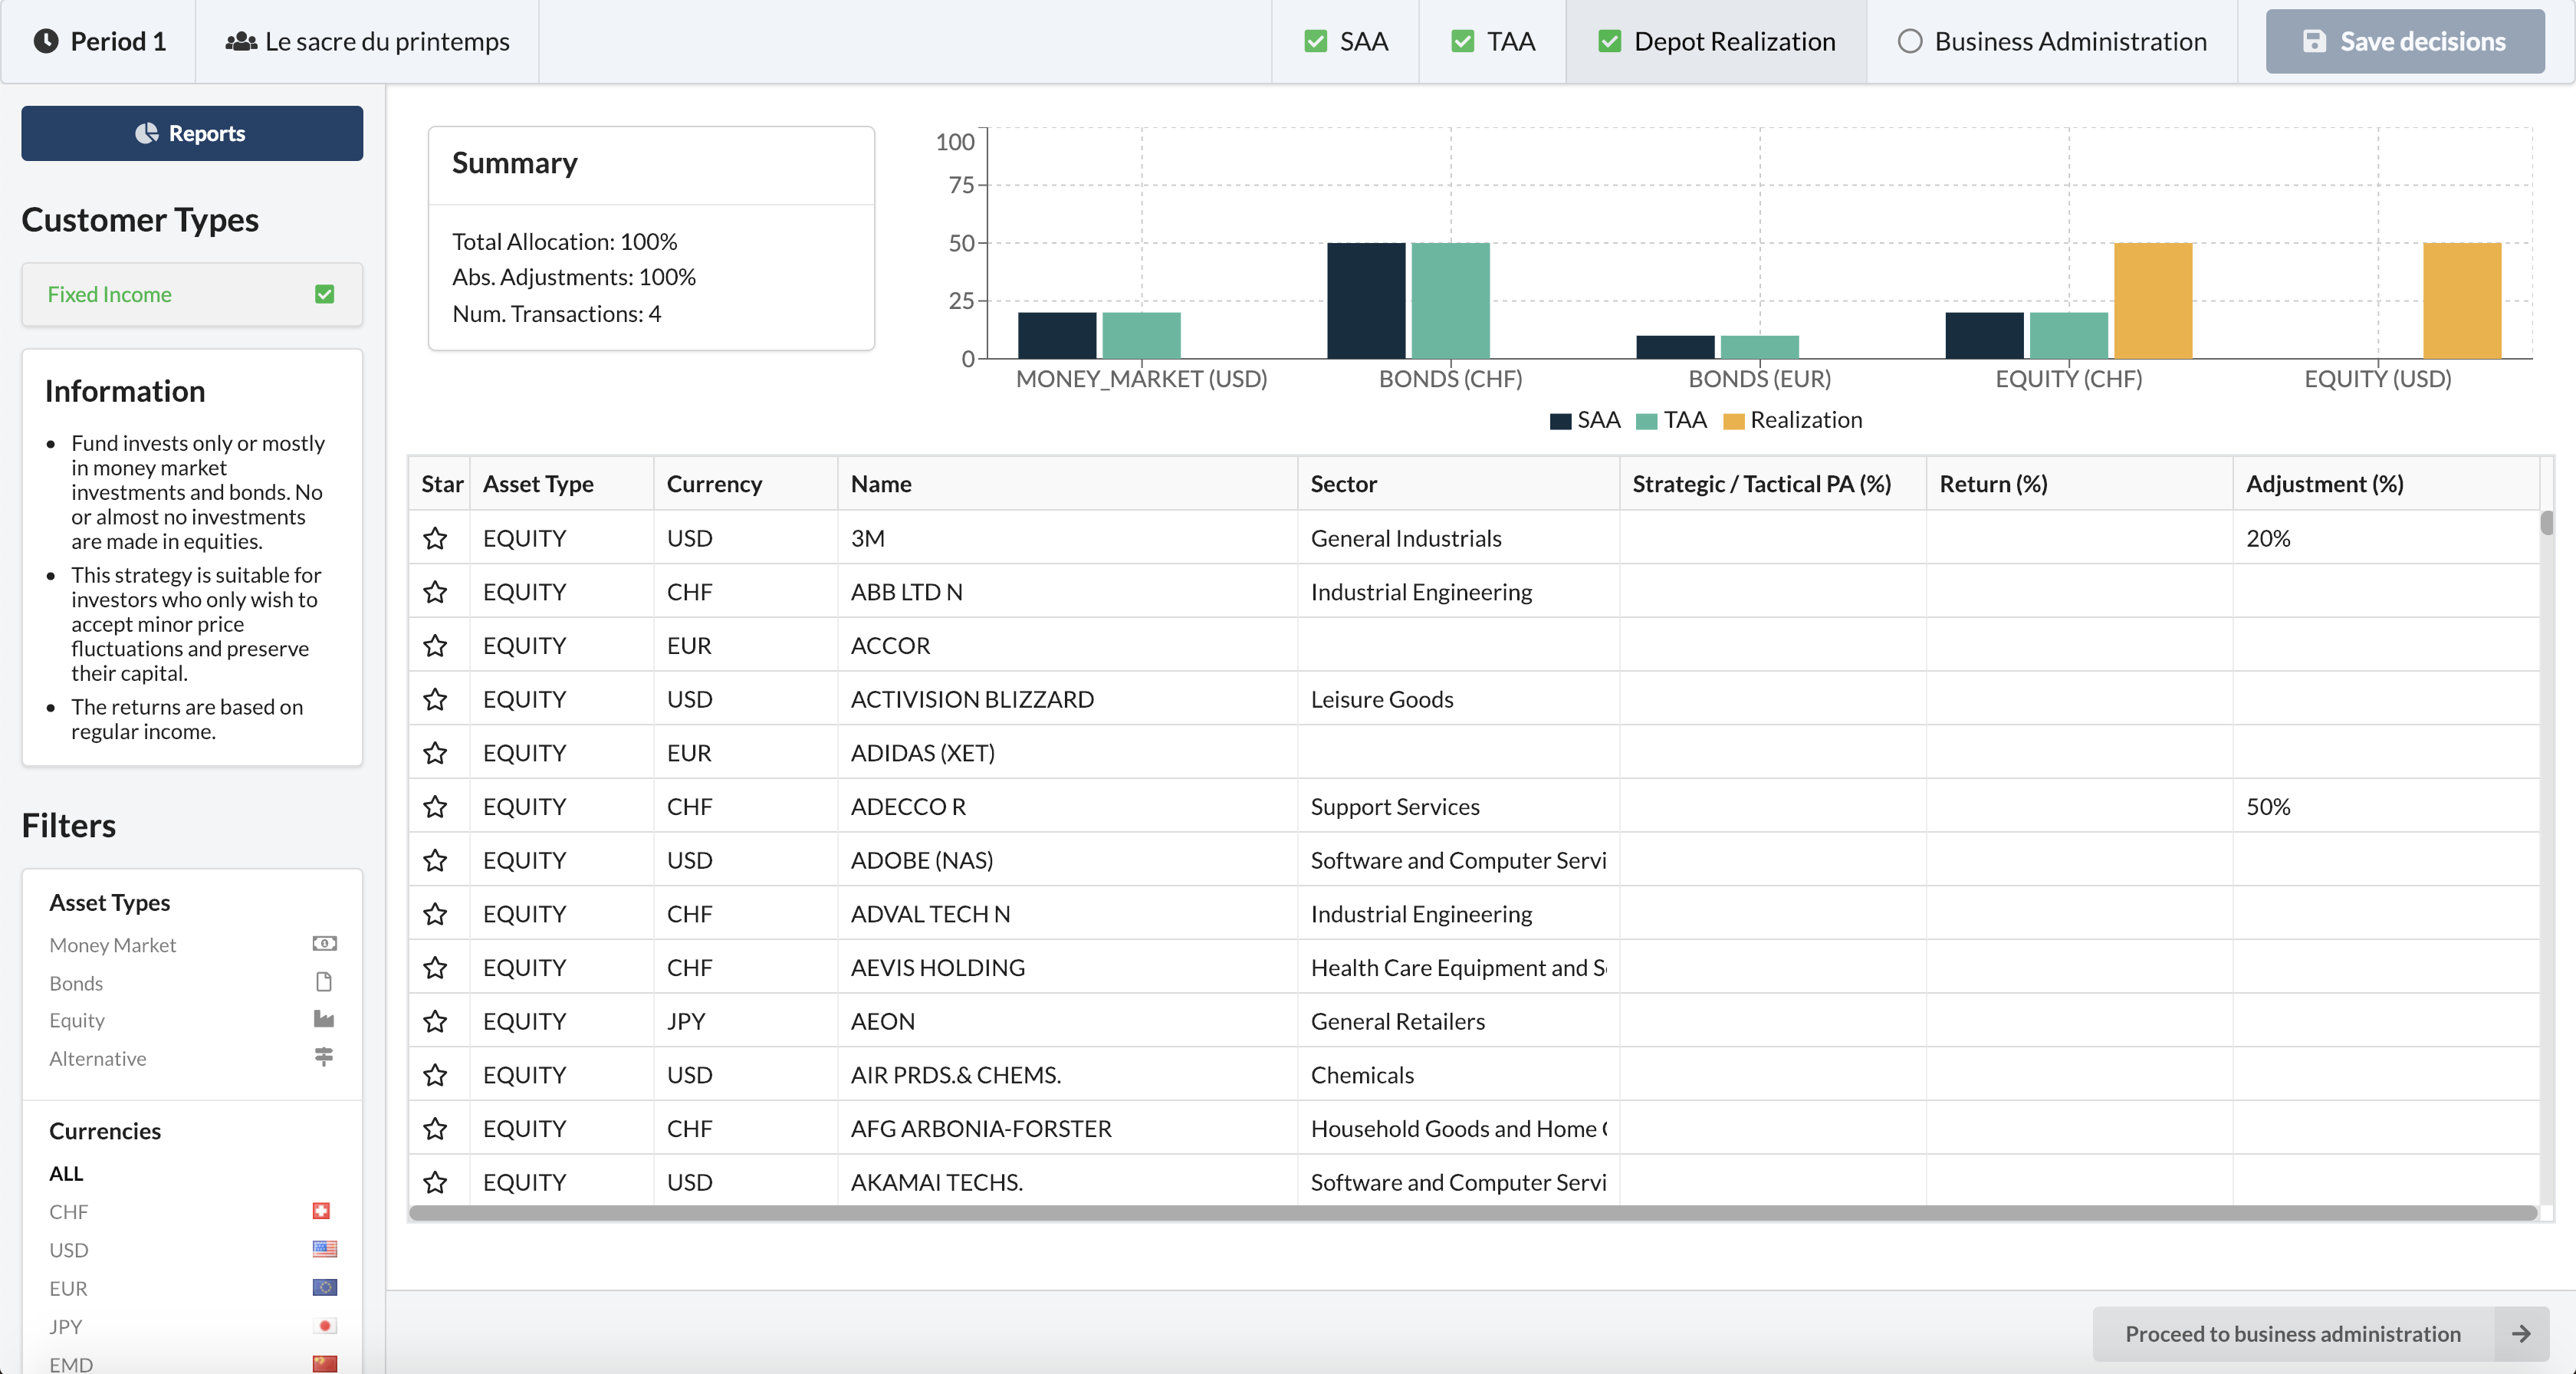
\includegraphics[scale=0.2]{img/application-overview/teams/depot_realization.png}
\end{center}

\subsubsection{Business Administration}
\begin{center}
  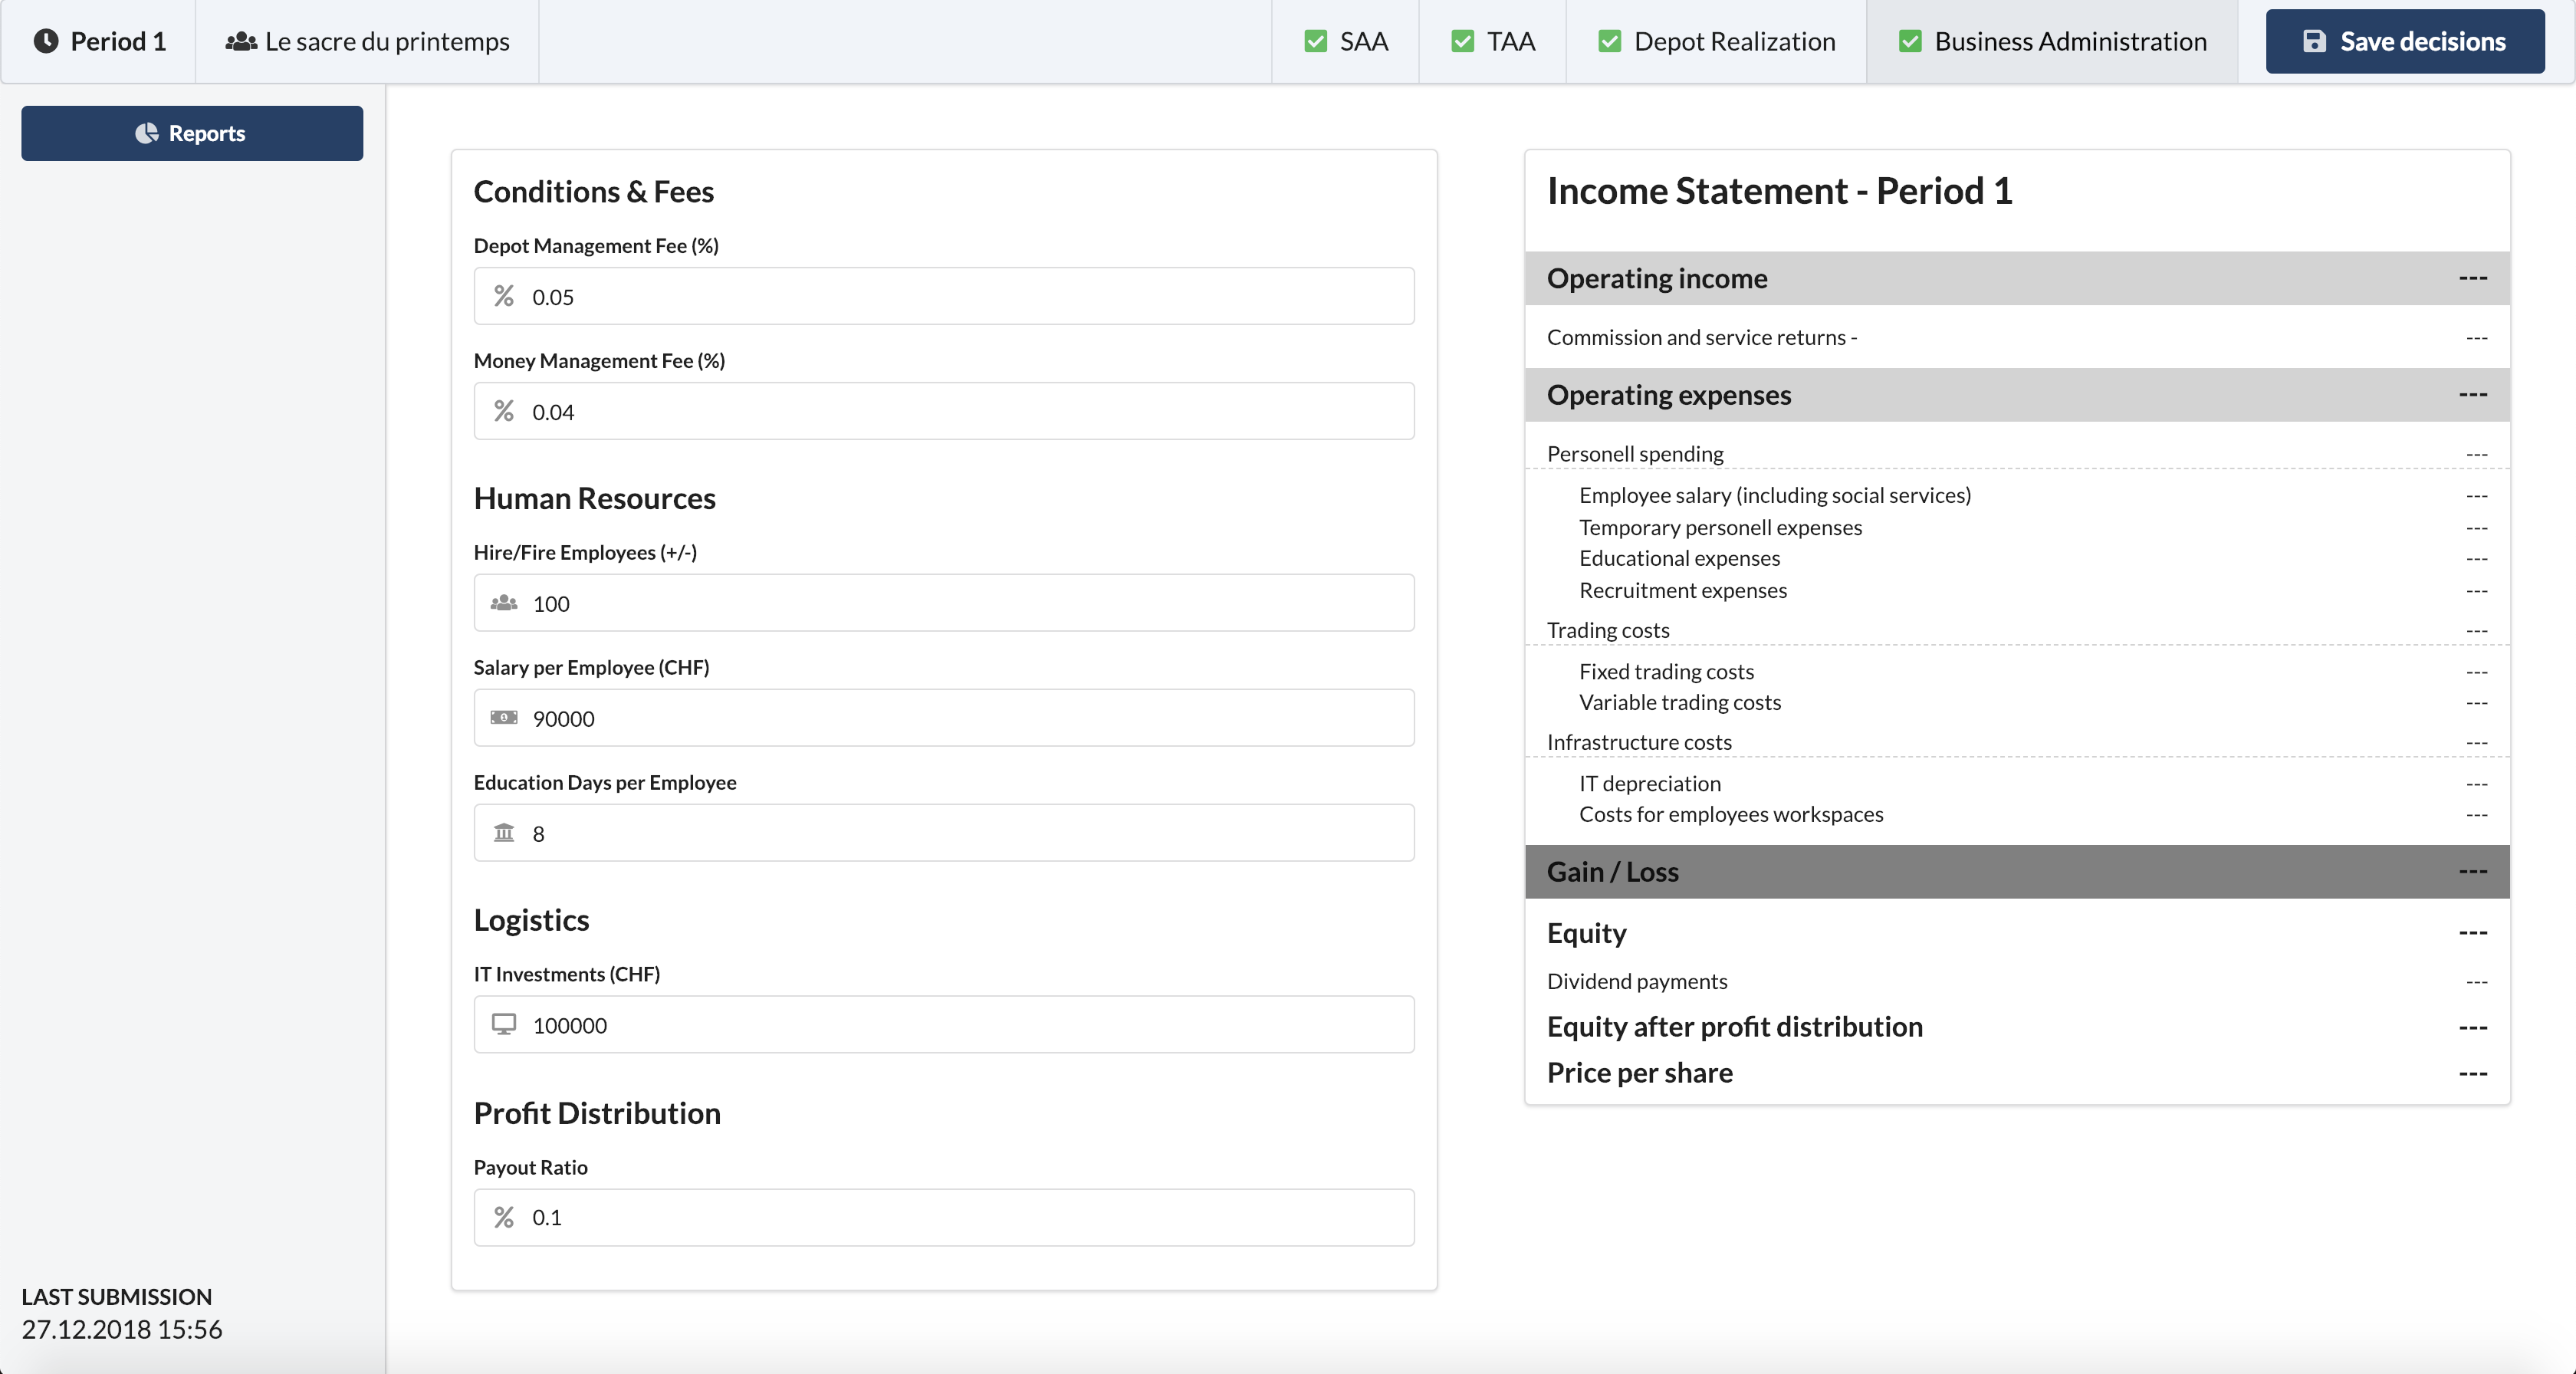
\includegraphics[scale=0.2]{img/application-overview/teams/business.png}
\end{center}
